%% LyX 2.3.6.2 created this file.  For more info, see http://www.lyx.org/.
%% Do not edit unless you really know what you are doing.
\documentclass[english,aspectratio=169]{beamer}
\usepackage{mathptmx}
\usepackage{eulervm}
\usepackage[T1]{fontenc}
\usepackage[latin9]{inputenc}
\usepackage{babel}
\usepackage{amstext}
\usepackage{amssymb}
\usepackage{graphicx}
\usepackage{ifthen}
\usepackage{xcolor}
\usepackage{comment}
\usepackage{xspace}
\usepackage{tikz}
\usetikzlibrary{tikzmark}
\usetikzlibrary{calc}
\usepackage{pgfplots}
\usepackage{booktabs}
\usepackage{bbm}

\ifx\hypersetup\undefined
  \AtBeginDocument{%
    \hypersetup{unicode=true,pdfusetitle,
 bookmarks=true,bookmarksnumbered=false,bookmarksopen=false,
 breaklinks=false,pdfborder={0 0 0},pdfborderstyle={},backref=false,colorlinks=true,
 allcolors=NYUPurple,urlcolor=LightPurple}
  }
\else
  \hypersetup{unicode=true,pdfusetitle,
 bookmarks=true,bookmarksnumbered=false,bookmarksopen=false,
 breaklinks=false,pdfborder={0 0 0},pdfborderstyle={},backref=false,colorlinks=true,
 allcolors=NYUPurple,urlcolor=LightPurple}
\fi

\makeatletter

%%%%%%%%%%%%%%%%%%%%%%%%%%%%%% LyX specific LaTeX commands.
%% Because html converters don't know tabularnewline
\providecommand{\tabularnewline}{\\}

%%%%%%%%%%%%%%%%%%%%%%%%%%%%%% Textclass specific LaTeX commands.
% this default might be overridden by plain title style
\newcommand\makebeamertitle{\frame{\maketitle}}%
% (ERT) argument for the TOC
\AtBeginDocument{%
  \let\origtableofcontents=\tableofcontents
  \def\tableofcontents{\@ifnextchar[{\origtableofcontents}{\gobbletableofcontents}}
  \def\gobbletableofcontents#1{\origtableofcontents}
}


% %%%%%%%%%%%%%%%%%%%%%%%%%%%%%% LyX specific LaTeX commands.
% %% Because html converters don't know tabularnewline
% \providecommand{\tabularnewline}{\\}

% %%%%%%%%%%%%%%%%%%%%%%%%%%%%%% Textclass specific LaTeX commands.
% % this default might be overridden by plain title style
% \newcommand\makebeamertitle{\frame{\maketitle}}%
% % (ERT) argument for the TOC
% \AtBeginDocument{%
%   \let\origtableofcontents=\tableofcontents
%   \def\tableofcontents{\@ifnextchar[{\origtableofcontents}{\gobbletableofcontents}}
%   \def\gobbletableofcontents#1{\origtableofcontents}
% }

%%%%%%%%%%%%%%%%%%%%%%%%%%%%%% User specified LaTeX commands.
\usetheme{CambridgeUS} 
\beamertemplatenavigationsymbolsempty


% Set Color ==============================
\definecolor{NYUPurple}{RGB}{87,6,140}
\definecolor{LightPurple}{RGB}{165,11,255}


\setbeamercolor{title}{fg=NYUPurple}
%\setbeamercolor{frametitle}{fg=NYUPurple}
\setbeamercolor{frametitle}{fg=NYUPurple}

\setbeamercolor{background canvas}{fg=NYUPurple, bg=white}
\setbeamercolor{background}{fg=black, bg=NYUPurple}

\setbeamercolor{palette primary}{fg=black, bg=gray!30!white}
\setbeamercolor{palette secondary}{fg=black, bg=gray!20!white}
\setbeamercolor{palette tertiary}{fg=gray!20!white, bg=NYUPurple}

\setbeamertemplate{headline}{}

\setbeamercolor{parttitle}{fg=NYUPurple}
\setbeamercolor{sectiontitle}{fg=NYUPurple}
\setbeamercolor{sectionname}{fg=NYUPurple}
\setbeamercolor{section page}{fg=NYUPurple}

\AtBeginSection[]{
  % \begin{frame}
  %   \frametitle{Table of Contents}
  %   \tableofcontents[currentsection]
  % \end{frame}

  \begin{frame}
  \vfill
  \centering
  \begin{beamercolorbox}[sep=8pt,center,shadow=true,rounded=true]{title}
    \usebeamerfont{title}\insertsectionhead\par%
  \end{beamercolorbox}
  \vfill
  \end{frame}
}

\makeatother

\input ../macros

\begin{document}
\global\long\def\reals{\mathbf{R}}%
 
\global\long\def\integers{\mathbf{Z}}%
 
\global\long\def\naturals{\mathbf{N}}%
 
\global\long\def\rationals{\mathbf{Q}}%
 
\global\long\def\ca{\mathcal{A}}%
 
\global\long\def\cb{\mathcal{B}}%
 
\global\long\def\cc{\mathcal{C}}%
 
\global\long\def\cd{\mathcal{D}}%
 
\global\long\def\ce{\mathcal{E}}%
 
\global\long\def\cf{\mathcal{F}}%
 
\global\long\def\cg{\mathcal{G}}%
 
\global\long\def\ch{\mathcal{H}}%
 
\global\long\def\ci{\mathcal{I}}%
 
\global\long\def\cj{\mathcal{J}}%
 
\global\long\def\ck{\mathcal{K}}%
 
\global\long\def\cl{\mathcal{L}}%
 
\global\long\def\cm{\mathcal{M}}%
 
\global\long\def\cn{\mathcal{N}}%
 
\global\long\def\co{\mathcal{O}}%
 
\global\long\def\cp{\mathcal{P}}%
 
\global\long\def\cq{\mathcal{Q}}%
 
\global\long\def\calr{\mathcal{R}}%
 
\global\long\def\cs{\mathcal{S}}%
 
\global\long\def\ct{\mathcal{T}}%
 
\global\long\def\cu{\mathcal{U}}%
 
\global\long\def\cv{\mathcal{V}}%
 
\global\long\def\cw{\mathcal{W}}%
 
\global\long\def\cx{\mathcal{X}}%
 
\global\long\def\cy{\mathcal{Y}}%
 
\global\long\def\cz{\mathcal{Z}}%
 
\global\long\def\ind#1{\mathbbm{1}[#1]}%
 %\newcommand{\pr}{P}
\global\long\def\pr{\mathbb{P}}%
 
\global\long\def\predsp{\cy}%
 %{\hat{\cy}}
\global\long\def\outsp{\cy}%

\global\long\def\prxy{P_{\cx\times\cy}}%
 
\global\long\def\prx{P_{\cx}}%
 
\global\long\def\prygivenx{P_{\cy\mid\cx}}%
 %\newcommand{\ex}{E}
\global\long\def\ex{\mathbb{E}}%
 
\global\long\def\var{\textrm{Var}}%
 
\global\long\def\cov{\textrm{Cov}}%
 
\global\long\def\sgn{\textrm{sgn}}%
 
\global\long\def\sign{\textrm{sign}}%
 
\global\long\def\kl{\textrm{KL}}%
 
\global\long\def\law{\mathcal{L}}%
 
\global\long\def\eps{\varepsilon}%
 
\global\long\def\as{\textrm{ a.s.}}%
 
\global\long\def\io{\textrm{ i.o.}}%
 
\global\long\def\ev{\textrm{ ev.}}%
 
\global\long\def\convd{\stackrel{d}{\to}}%
 
\global\long\def\eqd{\stackrel{d}{=}}%
 
\global\long\def\del{\nabla}%
 
\global\long\def\loss{\ell}%
 
\global\long\def\risk{R}%
 
\global\long\def\emprisk{\hat{R}}%
 
\global\long\def\lossfnl{L}%
 
\global\long\def\emplossfnl{\hat{L}}%
 
\global\long\def\empminimizer#1{\hat{#1}^{*}}%
 
\global\long\def\minimizer#1{#1^{*}}%
\global\long\def\optimizer#1{#1^{*}}%
 
\global\long\def\etal{\textrm{et. al.}}%
 
\global\long\def\tr{\operatorname{tr}}%

\global\long\def\trace{\operatorname{trace}}%
 
\global\long\def\diag{\text{diag}}%
 
\global\long\def\rank{\text{rank}}%
 
\global\long\def\linspan{\text{span}}%
 
\global\long\def\spn{\text{span}}%
 
\global\long\def\proj{\text{Proj}}%
 
\global\long\def\argmax{\operatornamewithlimits{arg\, max}}%
 
\global\long\def\argmin{\operatornamewithlimits{arg\, min}}%

\global\long\def\bfx{\mathbf{x}}%
 
\global\long\def\bfy{\mathbf{y}}%
 
\global\long\def\bfl{\mathbf{\lambda}}%
 
\global\long\def\bfm{\mathbf{\mu}}%
 
\global\long\def\calL{\mathcal{L}}%

\global\long\def\vw{\boldsymbol{w}}%
 
\global\long\def\vx{\boldsymbol{x}}%
 
\global\long\def\vxi{\boldsymbol{\xi}}%
 
\global\long\def\valpha{\boldsymbol{\alpha}}%
 
\global\long\def\vbeta{\boldsymbol{\beta}}%
 
\global\long\def\vsigma{\boldsymbol{\sigma}}%
\global\long\def\vtheta{\boldsymbol{\theta}}%
 
\global\long\def\vd{\boldsymbol{d}}%
 
\global\long\def\vs{\boldsymbol{s}}%
 
\global\long\def\vt{\boldsymbol{t}}%
 
\global\long\def\vh{\boldsymbol{h}}%
 
\global\long\def\ve{\boldsymbol{e}}%
 
\global\long\def\vf{\boldsymbol{f}}%
 
\global\long\def\vg{\boldsymbol{g}}%
 
\global\long\def\vz{\boldsymbol{z}}%
 
\global\long\def\vk{\boldsymbol{k}}%
 
\global\long\def\va{\boldsymbol{a}}%
 
\global\long\def\vb{\boldsymbol{b}}%
 
\global\long\def\vv{\boldsymbol{v}}%
 
\global\long\def\vy{\boldsymbol{y}}%

\global\long\def\dom{\textrm{\textbf{dom} }}%
\global\long\def\rank{\text{\textbf{rank }}}%
\global\long\def\conv{\textrm{\textbf{conv} }}%
\global\long\def\relint{\text{\textbf{relint }}}%
\global\long\def\aff{\text{\textbf{aff }}}%

\global\long\def\hil{\ch}%
 
\global\long\def\rkhs{\hil}%
 
\global\long\def\ber{\text{Ber}}%

\global\long\def\softmax{\text{Softmax}}%

\title[CSCI-GA 2565]{Probabilistic models - Bayesian Methods}
\author{Mengye Ren}
\date{Oct 17, 2023}
\institute{NYU}

% \makebeamertitle
\maketitle
\mode<article>{Just in article version}

% \begin{frame}{Contents}
% \tableofcontents{}
% \end{frame}


\section{Overview}
\begin{frame}
{Why probabilistic modeling?}
\begin{itemize}
\item A unified framework that covers many models, \eg linear regression, logistic regression
\item Learning as \textbf{statistical inference}
\item Principled ways to incorporate your belief on the data generating distribution (inductive biases)
\end{itemize}
\end{frame}

\begin{frame}
{Two ways of generating data}
\begin{itemize}
\item Two ways to model how the data is generated:
\pause
\begin{itemize}
\item \textbf{Conditional}: $p(y\mid x)$
\item \textbf{Generative}: $p(x, y)$
\end{itemize}
\pause
\item How to estimate the parameters of our model? Maximum likelihood estimation.
\pause
\item Compare and contrast conditional and generative models.
\end{itemize}
\end{frame}

\section{Conditional models}
\subsection{Recap: linear regression}

\begin{frame}{Linear regression}
Linear regression is one of the most important methods in machine learning and statistics.

\textbf{Goal}:  Predict a real-valued \textbf{target} $y$ (also called {response})
from a vector of \textbf{features} $x$ (also called {covariates}).
\pause

\textbf{Examples}:
\begin{itemize}
\item Predicting house price given location, condition, build year etc.
\item Predicting medical cost of a person given age, sex, region, BMI etc.
\item Predicting age of a person based on their photos.
\end{itemize}
\end{frame}

\begin{frame}{Problem setup}
\begin{description}
\item[Data] Training examples $\mathcal{D} = \{(x^{(n)}, y^{(n)})\}_{n=1}^N$,
where $x \in \mathbb{R}^d$ and $y \in \mathbb{R}$.
\pause{}

\item[Model] A \emph{linear} function $h$ (parametrized by $\theta$)
to predict $y$ from $x$:
\begin{align}
h(x) = \sum_{i=0}^d \theta_i x_i = \theta^T x,
\end{align}
where $\theta \in \mathbb{R}^d$ are the \textbf{parameters} (also called weights).
\end{description}
\pause{}

Note that
\begin{itemize}
\item We incorporate the \textbf{bias term} (also called the intercept term) into $x$ (i.e. $x_0 = 1$).
\item We use superscript to denote the example id and
    subscript to denote the dimension id.
\end{itemize}
\end{frame}

\begin{frame}{Parameter estimation}
\begin{description}
\item[Loss function]
We estimate $\theta$ by minimizing the \textbf{squared loss} (the least square method):
\begin{align}
\label{eqn:mse}
J(\theta) = \frac{1}{N}\sum_{n=1}^N \p{y^{(n)} - \theta^T x^{(n)}}^2 .
\;\;\; \text{(empirical risk)}
\end{align}
\pause{}

\item[Matrix form]
\begin{itemize}
\item Let $X \in \mathbb{R}^{N \times d}$ be the \textbf{design matrix}
whose rows are input features.
\item Let $\by \in \mathbb{R}^N$ be the vector of all targets.
\pause{}

\item We want to solve
\begin{align}
\hat{\theta} = \argmin_\theta (X\theta - \by)^T (X\theta - \by) .
\end{align}
\end{itemize}
\pause{}

\item[Solution]
Closed-form solution: $\hat{\theta} = (X^TX)^{-1}X^T\by$.
\end{description}
\pause{}

\begin{block}{Review questions}
\begin{itemize}
\item Derive the solution for linear regression.
\item What if $X^TX$ is not invertible?
\end{itemize}
\end{block}
\end{frame}

\begin{frame}{Review}
We've seen
\begin{itemize}
\item Linear regression: response is a linear function of the inputs
\item Estimate parameters by minimize the squared loss
\end{itemize}
\pause{}

But...
\begin{itemize}
\item Why squared loss is a reasonable choice for regression problems?
\item What assumptions are we making on the data? (\textcolor{blue}{inductive bias})
\end{itemize}
\pause{}

Next,
\begin{itemize}
\item Derive linear regression from a \textcolor{blue}{probabilistic modeling perspective}.
\end{itemize}
\end{frame}

\subsection{A probabilistic view of linear regression}
\begin{frame}
{Assumptions in linear regression}
\pause
\begin{itemize}
\item $x$ and $y$ are related through a linear function:
\begin{align}
y = \theta^Tx + \epsilon,
\end{align}
where $\epsilon$ is the \textbf{residual error} capturing all unmodeled effects (\eg noise).
\pause{}

\item The errors are  distributed $iid$ (independently and identically distributed):
\begin{align}
\epsilon \sim \mathcal{N}(0, \sigma^2) .
\end{align}
\end{itemize}
\pause{}

What's the distribution of $Y\mid X=x$?
\pause{}
\begin{align}
p(y\mid x \tikzmark{sc} {\color{blue};} \theta) = \mathcal{N}(\theta^Tx, \sigma^2) . 
\end{align}
Imagine putting a Gaussian bump around the output of the linear predictor.
\pause{}

%\begin{commentbox}[blue]
% \node[expl,text width=5cm] (sc_desc) at(12.5,2.5cm) {
%\small{$\theta$ as a fixed parameter vs a variable (more on this next time!).}
% };
% \draw[arrow] (sc_desc) to [in=90,out=180] ([yshift=1ex]{pic cs:sc});
%\end{commentbox}
\end{frame}

\begin{frame}
{Maximum likelihood estimation (MLE)}
\onslide<1->{
Given a probabilistic model and a dataset $\mathcal{D}$,
how to estimate the model parameters $\theta$?
}

\onslide<2->{
The \textbf{maximum likelihood principle} says that we should maximize the (conditional) likelihood of the data:
}
\begin{align}
\onslide<2->{L(\theta) &\eqdef p(\mathcal{D}; \theta) \\}
\onslide<3->{&= \prod_{n=1}^N p(y^{(n)}\mid x^{(n)}; \theta) .  && \text{(examples are distributed \emph{iid})}}
\end{align}

\onslide<4->{
In practice, we maximize the \tikzmark{txt} \textbf{\textcolor{blue}{log} likelihood} $\ell(\theta)$,
or equivalently, minimize the negative log likelihood (NLL).
}

%\onslide<5->{
%\begin{commentbox}[blue]
% \node[expl,text width=6cm] (txt_desc) at(9,-0cm) {
%\small{$L(\theta_1) \leq L(\theta_2) \implies \log L(\theta_1) \leq \log L(\theta_2)$}
% };
% \draw[arrow] (txt_desc) to [in=270,out=180] ([xshift=1ex,yshift=-1ex]{pic cs:txt});
%\end{commentbox}
%}
\end{frame}

\begin{frame}
{MLE for linear regression}
\onslide<1->{
Let's find the MLE solution for our model.
Recall that $Y\mid X=x \sim  \mathcal{N}(\theta^Tx, \sigma^2)$.
}
\begin{align}
\onslide<2->{
\ell(\theta) &\eqdef \log L(\theta) \\
                   &= \log \prod_{n=1}^N p(y^{(n)}\mid x^{(n)}; \theta) \\
                   &= \sum_{n=1}^N \log p(y^{(n)}\mid x^{(n)}; \theta) \\}
\onslide<3->{                  
                   &= \sum_{n=1}^N \log \frac{1}{\sqrt{2\pi}\sigma}
                   \exp\left( -\frac{
                       \left( y^{(n)} - \theta^Tx^{(n)} \right)^2}
                       {2\sigma^2} 
                   \right) \\}
\onslide<4->{                   
                   &= \tikzmark{first} {\color<5->{blue} N\log\frac{1}{\sqrt{2\pi}\sigma} } 
                         \tikzmark{minus} {\color<6->{red} - }
                         \tikzmark{multi} {\color<5->{blue} \frac{1}{2\sigma^2} }
                         \tikzmark{sum} {\color<6->{red} \sum_{n=1}^{N}  \left( y^{(n)} - \theta^Tx^{(n)} \right)^2 }
}
\end{align}

%\onslide<5->{
%\begin{commentbox}[blue]
% \node[expl,text width=4cm] (first_desc) at(2,2cm) {
%\small{does not depend on $\theta$}
% };
% \draw[arrow] (first_desc) to [in=270,out=270] ([xshift=2ex,yshift=-1ex]{pic cs:first});
%\end{commentbox}
%}

%\onslide<6->{
%\begin{commentbox}[red]
% \node[expl,text width=3cm] (ls) at(13.5,3cm) {
%\small{minimizing squared loss!}
% };
% \draw[arrow] (ls) to [in=90,out=180] ([xshift=6ex,yshift=2ex]{pic cs:sum});
%\end{commentbox}
%}
\end{frame}

\begin{frame}
{Gradient of the likelihood}
Recall that we obtained the normal equation by setting the derivative of the squared loss to zero. Now let's compute the derivative of the likelihood w.r.t. the parameters.
\begin{align}
\onslide<1->{
\ell(\theta) &= N\log\frac{1}{\sqrt{2\pi}\sigma} 
                      - 
                       \frac{1}{2\sigma^2}
                       \sum_{n=1}^{N}  \left( y^{(n)} - \theta^Tx^{(n)} \right)^2 \\
}
\onslide<2->{
\frac{\partial \ell}{\partial \theta_i} &= -\frac{1}{\sigma^2}
               \sum_{n=1}^N (y^{(n)} - \tikzmark{linear-term}{ \color<3->{blue} \theta^T x^{(n)} }) x^{(n)}_i  .
               }
\end{align}
% \onslide<3->{
% \begin{commentbox}[blue]
% \node[expl,text width=3cm] (linear-mean) at(11,-0cm) {
% $\mathbb{E} [Y\mid X=x^{(n)}] $
% };
% \draw[arrow] (linear-mean) to [in=270,out=180] ([xshift=2ex,yshift=-1ex]{pic cs:linear-term});
% \end{commentbox}

% (Spoiler: we will see this form again.)
% }
\end{frame}

\begin{frame}
{Review}
We've seen
\begin{itemize}
\item Linear regression assumes that $Y\mid X=x$ follows a Gaussian distribution
\item MLE of linear regression is equivalent to the least square method
\end{itemize}
\pause{}

However,
\begin{itemize}
\item Sometimes Gaussian distribution is not a reasonable assumption, \eg classification
\item Can we use the same modeling approach for other prediction tasks?
\end{itemize}
\pause{}

Next,
\begin{itemize}
\item Derive \textcolor{blue}{logistic regression} for classification.
\end{itemize}
\end{frame}

\subsection{Logistic regression}
\begin{frame}
{Assumptions in logistic regression}
\onslide<1->{
Consider binary classification where $Y \in \{0, 1\}$.
What should be the distribution $Y\mid X=x$?
}

\onslide<2->{
We model $p(y\mid x)$ as a \textcolor{blue}{Bernoulli} distribution:
\begin{align}
p(y\mid x) = h(x)^y (1-h(x))^{1-y} .
\end{align}
}

\onslide<3->{
How should we parameterize $h(x)$?
}
\begin{itemize}
\onslide<4->{
\item What is $p(y=1\mid x)$ and $p(y=0\mid x)$?
}
\onslide<5->{ $h(x) \in (0,1)$. }
\onslide<6->{
\item What is the mean of $Y\mid X=x$?
}
\onslide<7->{ $h(x)$. (Think how we parameterize the mean in linear regression) }
\onslide<8->{
\item Need a function $f$ to map the linear predictor $\theta^Tx$ in $\mathbb{R}$ to $(0,1)$:
\begin{align}
f(\eta) = \frac{1}{1 + e^{-\eta}} && \text{\color{blue}logistic function}
\end{align}
}
\end{itemize}
\end{frame}

\begin{frame}
{Logistic regression}
\begin{columns}
\begin{column}{0.5\textwidth}  %%<--- here
\begin{center}
    \begin{tikzpicture}
    \begin{axis}[
        title={$f(\eta) = \frac{1}{1+e^{-\eta}}$}, xlabel={$\eta$}, ylabel={$f(\eta)$},
        width=\textwidth
    ]
    \addplot [
        blue, thick,
        domain=-10:10,
        samples=500,
    ]
    { 1 / (1 + exp(-x)) };
    \end{axis}
    \end{tikzpicture}
\end{center}
\end{column}

\begin{column}{0.5\textwidth}
\begin{itemize}
\item $p(y\mid x) = \text{Bernoulli}(f(\theta^T x))$.
\pause
\item When do we have $p(y=1\mid x) = 1$ and $p(y=0\mid x) = 1$?
\pause
\item \textcolor{green}{Exercise}: show that the \textbf{log odds} is
\begin{align}
\log \frac{p(y=1\mid x)}{p(y=0\mid x)}=\theta^Tx . \\
\implies \text{linear decision boundary}
\end{align}
\pause
\item How do we extend it to multiclass classification? (more on this later)
\end{itemize}
\end{column}
\end{columns}
\end{frame}

\begin{frame}
{MLE for logistic regression}
\onslide<1->{
Similar to linear regression, let's estimate $\theta$ by maximizing the conditional log likelihood.
}
\begin{align}
\onslide<2->{\ell(\theta) &= \sum_{n=1}^N \log p(y^{(n)} \mid x^{(n)}; \theta) \\}
\onslide<3->{&= \sum_{n=1}^N y^{(n)}\log f(\theta^T x^{(n)}) + (1-y^{(n)})\log (1 - f(\theta^T x^{(n)}))}
\end{align}

\onslide<4->{
\begin{itemize}
\item Closed-form solutions are not available.
\item But, the likelihood is concave---\textcolor{blue}{gradient ascent} gives us the unique optimal solution.
\begin{align}
\theta := \theta + \alpha \nabla_\theta \ell(\theta) .
\end{align}
\end{itemize}
}
\end{frame}

\begin{frame}
{Gradient descent for logistic regression}
\onslide<1->{
\begin{block}{Math review: Chain rule}
If $z$ depends on $y$ which itself depends on $x$, \eg $z=\p{y(x)}^2$,
then
$
\frac{dz}{dx} = \frac{dz}{dy} \frac{dy}{dx}
$.
\end{block}
}
\onslide<2->{
Likelihood for a single example: $\ell^n=y^{(n)}\log f(\theta^T x^{(n)}) + (1-y^{(n)})\log (1 - f(\theta^T x^{(n)}))$.
}

\begin{align}
\onslide<3->{
\frac{\partial \ell^n}{\partial \theta_i}  &= \frac{\partial \ell^n}{\partial f^n}\frac{\partial f^n}{\partial \theta_i} \\
}
\onslide<4->{
&= \left( \frac{y^{(n)}}{f^n} - \frac{1-y^{(n)}}{1-f^n} \right) 
      \frac{\partial f^n}{\partial \theta_i}  & \frac{d}{dx}\ln x = \frac{1}{x} \\
}
\onslide<5->{
&= \left( \frac{y^{(n)}}{f^n} - \frac{1-y^{(n)}}{1-f^n} \right)
      \left( f^n (1 - f^n) x^{(n)}_i \right) & \text{\textcolor{green}{Exercise}: apply chain rule to $\frac{\partial f^n}{\partial \theta_i}$} \\
&= (y^{(n)} - f^n) x^{(n)}_i & \text{simplify by algebra}
}
\end{align}
\onslide<6->{
The full gradient is thus $\frac{\partial \ell}{\partial \theta_i} = \sum_{n=1}^N (y^{(n)} - f(\theta^T x^{(n)})) x^{(n)}_i$.
}
\end{frame}

\begin{frame}
{A closer look at the gradient}
\onslide<1->{
\begin{align}
\frac{\partial \ell}{\partial \theta_i} = \sum_{n=1}^N (y^{(n)} - \tikzmark{f}{ \color<2->{blue} f(\theta^T x^{(n)}) } ) x^{(n)}_i
\end{align}
}
%\onslide<2->{
%\begin{commentbox}[blue]
% \node[expl,text width=3cm] (mean) at(11,2cm) {
%$\mathbb{E} [Y\mid X=x^{(n)}] $
% };
% \draw[arrow] (mean) to [in=90,out=180] ([xshift=2ex,yshift=2ex]{pic cs:f});
%\end{commentbox}
%}
\onslide<3->{
\begin{itemize}
\item Does this look familiar?
\item Our derivation for linear regression and logistic regression are quite similar...
\item Next, a more general family of models.
\end{itemize}
}
\end{frame}

\subsection{Generalized Linear Models}
\begin{frame}
{Compare linear regression and logistic regression}
\begin{table}
\begin{tabular}{lll}
\toprule
 & linear regression & logistic regression \\ 
 \midrule \pause
Combine the inputs & $\theta^T x$ (linear) & $\theta^T x$ (linear) \\ \pause
\textcolor{blue}{Output} & real & categorical \\
\textcolor{blue}{Conditional distribution} & Gaussian & Bernoulli \\ \pause
\textcolor{blue}{Transfer function} $f( \theta^T x )$ & identity & logistic \\ \pause
Mean $\mathbb{E}(Y\mid X=x; \theta)$ & $f( \theta^T x )$ & $f( \theta^T x )$ \\
\bottomrule
\end{tabular}
\end{table}
\pause
\begin{itemize}
\item $x$ enters through a linear function.
\item The main \textcolor{blue}{difference} between the formulations is due to different conditional distributions.
\item Can we generalize the idea to handle other output types, \eg positive integers?
\end{itemize}
\end{frame}

%\begin{frame}
%{Generalized linear models (GLM)}
%\onslide<1->{
%\textbf{Main idea}: use a class of distributions known as the \textbf{exponential family} as the response distribution.
%}
%
%\onslide<2->{
%The exponential family has the following form:
%\begin{align}
%p(y; \eta) = h(y)\exp(\tikzmark{eta}{\color<3->{blue}\eta}^T \tikzmark{ty}{\color<4->{red}T(y)} - \tikzmark{A}{\color<5->{green}A(\eta)})
%\end{align}
%}
%%
%%\begin{commentbox}[blue]
%%\onslide<3->{
%% \node[expl,text width=3cm] (np) at(3,0.5cm) {
%%natural parameters
%% };
%% \draw[arrow] (np) to [in=270,out=0] ([xshift=1ex,yshift=-1ex]{pic cs:eta});
%% }
%%\onslide<4->{
%% \node[expl,text width=3cm,draw=red,fill=red!20] (ss) at(11, 0.5cm) {
%%sufficient statistics
%%};
%% \draw[arrow,red] (ss) to [in=270,out=180] ([xshift=2ex,yshift=-1ex]{pic cs:ty});
%%}
%%\onslide<5->{
%% \node[expl,text width=3cm,draw=Green,fill=Green!20] (par) at(12,2cm) {
%%normalizer};
%% \draw[arrow,Green] (par) to [in=90,out=180] ([xshift=2ex,yshift=2ex]{pic cs:A});
%% }
%%\end{commentbox}
%%
%\begin{itemize}
%\onslide<6->{
%\item Many nice properties, \eg conjugate priors for Bayesian inference.
%\item \textbf{Useful property for this class}:
%\begin{align}
%& \mu \eqdef \mathbb{E}[Y] = \psi^{-1}(\eta), \;\; \eta = \psi(\mu) \\
%& \mu = A'(\eta)
%\end{align}
%}
%\onslide<7->{
%\item Example: Gaussian, Bernoulli, Poisson distribution.
%\item \textcolor{green}{Exercise}: find $\eta, T(y), A(\eta), h(y)$ for Gaussian distribution.
%}
%\end{itemize}
%
%\end{frame}

\begin{frame}
{Construct a generalized regression model}
\textbf{Task}: %build a model $h(x)$ to estimate $T(y)$ given some inputs $x$ ($T(y)=y$ in most examples).
    Given $x$, predict $p(y\mid x)$

%\textbf{Assumption}: an exponential family distribution is a good model for $Y\mid X$.
%\pause
\textbf{Modeling}:
\begin{itemize}
    \item Choose a parametric family of distributions $p(y;\theta)$ with parameters $\theta\in\Theta$
%\begin{align}
%Y\mid X=x; \theta \sim \text{ExponentialFamily}(\eta) \;\;\text{where}\;\; \eta = \theta^Tx.
%\end{align}
%\pause
\item Choose a transfer function that maps a linear predictor in $\BR$ to $\Theta$ 
\begin{align}
  \underbrace{x}_{\in\reals^{d}}\mapsto\underbrace{w^{T}x}_{\in\reals}\mapsto\pause\underbrace{f(w^{T}x)}_{\in\Theta}=\theta,
\end{align}
%\begin{itemize}
%\item An available choice is $\psi^{-1}$, which is the canonical link function.
%\end{itemize}
%\pause
\end{itemize}
{\bf Learning}: 
        MLE: $\hat{\theta}  \in \argmax_{\theta}\log p(\cd;\hat{\theta})$

{\bf Inference}:
 For prediction, use $x \to f(w^Tx)$  %= \mathbb{E}(Y\mid X=x) $.
\end{frame}

\begin{frame}
{Example: Construct Poisson regression}
Say we want to predict the number of people entering a restaurant in New York during lunch time.
\begin{itemize}
\item What features would be useful?
\item What's a good model for number of visitors (the \textcolor{blue}{output distribution})?
\end{itemize}
\pause

\begin{block}{Math review: Poisson distribution}
Given a random variable $Y \in {0, 1, 2, \ldots}$ following $\text{Poisson}(\lambda)$, we have
\begin{align}
p(Y=k; \lambda) = \frac{\lambda^ke^{-\lambda}}{k!} ,
\end{align}
where $\lambda > 0$ and $\mathbb{E}[Y] = \lambda$.
\end{block}
The Poisson distribution is usually used to model the number of events occurring during a fixed period of time. 
\end{frame}

\begin{frame}
{Example: Construct Poisson regression}

We've decided that $Y\mid X=x \sim \text{Poisson}(\tikzmark{poi-eta}\eta)$,
what should be the transfer function $f$?

$x$ enters {linearly:}
    $$
    x\mapsto\underbrace{w^{T}x}_{\reals}\mapsto\lambda=\underbrace{f(w^{T}x)}_{(0,\infty)}
    $$

Standard approach is to take
\[
f(w^{T}x)=\exp\left(w^{T}x\right).
\]

Likelihood of the full dataset $\cd=\left\{ (x_{1},y_{1}),\ldots,(x_{n},y_{n})\right\} $:
    \begin{align}
\log p(y_{i};\lambda_{i}) &= \left[y_{i}\log\lambda_{i}-\lambda_{i}-\log\left(y_{i}!\right)\right] \\
\log p(\cd;w) &= \sum_{i=1}^{n}\left[y_{i}\log\left[\exp\left(w^{T}x_{i}\right)\right]-\exp\left(w^{T}x_{i}\right)-\log\left(y_{i}!\right)\right]\\
 &= \sum_{i=1}^{n}\left[y_{i}w^{T}x_{i}-\exp\left(w^{T}x_{i}\right)-\log\left(y_{i}!\right)\right]
    \end{align}

\end{frame}

% \begin{frame}
% {Example: multinomial logistic regression}
% How to extend logistic regression to multiclass classification?

% \pause
% Output: Bernoulli distribution $\rightarrow$ \textcolor{blue}{categorical distribution}
% \begin{itemize}
% \item Parametrized by a probability vector $\theta=\left(\theta_{1},\ldots,\theta_{k}\right)\in\BR^{k}$:
% \begin{itemize}
% \item $\sum_{i=1}^{k}\theta_{i}=1$ and $\theta_{i}\ge0$ for $i=1,\ldots,k$
% %\item i.e. $\theta$ represents a \textbf{discrete distribution}) 
% \item So $\forall y\in\left\{ 1,\ldots,k\right\} $, $p(y)=\theta_{y}$.
% \end{itemize}
% \end{itemize}

% \item From each $x$, we compute a linear score function for each class:
% \[
% x\mapsto\left(\left\langle w_{1},x\right\rangle ,\ldots,\left\langle w_{k},x\right\rangle \right)\in\BR^{k},
% \]

% What's the transfer function that maps this $\BR^{k}$ vector into a probability?

%     The \textbf{softmax function}:
% \[
% \left(s_{1},\ldots,s_{k}\right)\mapsto\theta=\left(\frac{e^{s_{1}}}{\sum_{i=1}^{k}e^{s_{i}}},\ldots,\frac{e^{s_{k}}}{\sum_{i=1}^{k}e^{s_{i}}}\right).
% \]
% \end{frame}

\begin{frame}{Multinomial Logistic Regression}
\begin{itemize}
\item Say we want to get the predicted categorical distribution for a given
$x\in\reals^{d}$. 
\item First compute the scores $(\in\reals^{k})$ and then their softmax:
\textbf{
\[
x\mapsto\left(\left\langle w_{1},x\right\rangle ,\ldots,\left\langle w_{k},x\right\rangle \right)\mapsto\theta=\left(\frac{\exp\left(w_{1}^{T}x\right)}{\sum_{i=1}^{k}\exp\left(w_{i}^{T}x\right)},\ldots,\frac{\exp\left(w_{k}^{T}x\right)}{\sum_{i=1}^{k}\exp\left(w_{i}^{T}x\right)}\right)
\]
}
\end{itemize}

\pause{}
\begin{itemize}
\item We can write the conditional probability for any $y\in\left\{ 1,\ldots,k\right\} $
as
\[
p(y\mid x;w)=\frac{\exp\left(w_{y}^{T}x\right)}{\sum_{i=1}^{k}\exp\left(w_{i}^{T}x\right)}.
\]
\end{itemize}
\end{frame}

\begin{frame}
{Review}
Recipe for contructing a conditional distribution for prediction:
\begin{enumerate}
\item Define input and output space (as for any other model).
\item Choose the output distribution $p(y\mid x; \theta)$ based on the task %that belongs to the exponential family.
\item Choose the transfer function that maps $w^Tx$ to a $\Theta$.
\item (The formal family is called ``generalized linear models''.)
\end{enumerate}

Learning:\\
\begin{itemize}
\item Fit the model by maximum likelihood estimation.
\item Closed solutions do not exist in general, so we use gradient ascent.
\end{itemize}
\end{frame}

%\begin{frame}
%{MLE for GLM}
%\onslide<1->{
%Recall that the likelihood of the exponential family has the form
%\begin{align}
%\log p(y\mid x; \theta) = \eta^Ty - A(\eta) .
%\end{align}
%}
%
%\onslide<2->{
%Let's compute the gradient of the likelihood.
%}
%\begin{align}
%\onslide<2->{
%\nabla_\theta \ell(\theta) &= \sum_{n=1}^N \nabla_{\eta^n}\ell^n \nabla_{\theta}\eta^n
%   & \text{chain rule} \\
%}
%\onslide<3->{
%&= \sum_{n=1}^N  \left( y^{(n)} - \nabla_{\eta^n} A(\eta^n) \right) x^{(n)} 
%   & \eta^n = \theta^T x^{(n)} \\
%}
%\onslide<4->{
%&= {\color{blue}
%       \sum_{n=1}^N  \left( y^{(n)} - \mathbb{E}[Y \mid x^{(n)}; \theta] \right) x^{(n)} 
%      }
%      & A'(\eta) = \mu
%}
%\end{align}
%\onslide<5->{
%Same form as we've seen in linear regression and logistic regression.
%}
%\end{frame}

\section{Generative models}
\begin{frame}
{Review}
We've seen
\begin{itemize}
\item Model the conditional distribution $p(y\mid x; \theta)$ using generalized linear models.
\item (Previously) Directly map $x$ to $y$, \eg perceptron.
\end{itemize}

Next,
\begin{itemize}
\item Model the \textcolor{blue}{joint distribution} $p(x, y; \theta)$.
\item Predict the label for $x$ as $\argmax_{y\in \mathcal{Y}} p(x, y; \theta)$.
\end{itemize}
\end{frame}

\begin{frame}
{Generative modeling through the Bayes rule}
\onslide<1->{
Training:
}
\onslide<3->{
%\begin{commentbox}[blue]
% \node[expl,text width=3cm] (gen-expl) at(3,0cm) {
%to be parametrized
% };
% \draw[arrow] (gen-expl) to [in=90,out=0] ([xshift=1ex,yshift=2ex]{pic cs:gen});
%
% \node[expl,text width=3cm,draw=red,fill=red!20] (y-expl) at(10, 0cm) {
%class priors
%};
% \draw[arrow,red] (y-expl) to [in=90,out=180] ([xshift=1ex,yshift=2ex]{pic cs:y});
%\end{commentbox}
}
\begin{align}
\onslide<1->{
p(x,y)
}
\onslide<2->{
= {\tikzmark{gen}{\color<3->{blue}p(x\mid y)}\tikzmark{y}{\color<3->{red}p(y)}}
}
\end{align}

\onslide<4->{
Testing:
}
\begin{align}
\onslide<4->{
p(y\mid x)
}
\onslide<5->{
 &= \frac{p(x\mid y) p(y)}{p(x)} & \text{Bayes rule} \\
}
\onslide<6->{
\argmax_y p(y\mid x) &= \argmax_y p(x\mid y) p(y)
}
\end{align}
\end{frame}

\subsection{Naive Bayes models}
\subsubsection{Bernoulli Naive Bayes Models}
\begin{frame}
{Naive Bayes (NB) models}
Let's consider binary text classification (\eg fake vs genuine review) as a motivating example.
\pause

\textbf{Bag-of-words} representation of a document
\begin{itemize}
\item \text{[``machine'', ``learning'', ``is'', ``fun'', ``.'']}
\item $x_i \in \{0, 1\}$: whether the $i$-th word in our vocabulary exists in the input
\begin{align}
x = [x_1, x_2, \ldots, x_d] \;\; \text{ where } d = \text{vocabulary size}
\end{align}
\end{itemize}
\pause

What's the probability of a document $x$?
\pause
\begin{align}
p(x\mid y) &= p(x_1, \ldots, x_d \mid y) \\
&= p(x_1\mid y) p(x_2\mid y, x_1) p(x_3\mid y, x_2, x_1) \dots p(x_d\mid y, x_{d-1}, \ldots, x_1) & \text{chain rule} \\
&= \prod_{i=1}^d p(x_i\mid y, x_{<i})
\end{align}
\end{frame}

\begin{frame}
{Naive Bayes assumption}
\textbf{Challenge}: $p(x_i\mid y, x_{<i})$ is hard to model (and estimate), especially for large $i$.
\pause

Solution:
\begin{block}
{Naive Bayes assumption}
Features are \textbf{conditionally independent} given the label:
\begin{align}
p(x\mid y) = \prod_{i=1}^d p(x_i\mid y) .
\end{align}
\end{block}

A strong assumption in general, but works well in practice.
\end{frame}

\begin{frame}
{Parametrize $p(x_i\mid y)$ and $p(y)$}
For binary $x_i$, assume $p(x_i\mid y)$ follows Bernoulli distributions.
\begin{align}
p(x_i=1 \mid y=1) &= \theta_{i,1}, \;\; p(x_i=1 \mid y=0) = \theta_{i,0}  .
\end{align}
\pause
Similarly,
\begin{align}
p(y=1) = \theta_0 .
\end{align}
\pause
Thus,
\begin{align}
p(x,y) &= p(x\mid y) p(y) \\
&= p(y)\prod_{i=1}^d p(x_i\mid y) && \text{NB assumption} \\
&= p(y)\prod_{i=1}^d \theta_{i,y} \1\pc{x_i=1} + \p{1- \theta_{i,y}}\1\pc{x_i=0} 
\end{align}
Indicator function $\1\pc{\text{condition}}$ evaluates to 1 if ``condition'' is true and 0 otherwise. 
\end{frame}

\begin{frame}
{MLE for our NB model}
\onslide<1->{
We maximize the likelihood of the data $\prod_{n=1}^N p_\theta(\xn, \yn)$ (as opposed to the \emph{conditional} likelihood we've seen before).
}
\begin{align}
\onslide<2->{
    \frac{\partial}{\partial \theta_{j,1}}\ell &= \frac{\partial}{\partial \theta_{j,1}}
    \sum_{n=1}^N \sum_{i=1}^d \log \p{ \theta_{i,\yn} \1\pc{\xn_i=1} + \p{1- \theta_{i,\yn}}\1\pc{\xn_i=0} } 
+ \log p_{\theta_0}(\yn) \\
}
\onslide<3->{
&= \frac{\partial}{\partial \theta_{j,1}}
    \sum_{n=1}^N \log \p{ \theta_{j,\yn} \1\pc{\xn_j=1} + \p{1- \theta_{j,\yn}}\1\pc{\xn_j=0} } \qquad \text{ignore } i \neq j \\
}
\onslide<4->{
&= \sum_{n=1}^N \1\pc{ \yn=1 \wedge \xn_j=1 } \frac{1}{\theta_{j,1}} +
                            \1\pc{ \yn=1 \wedge \xn_j=0 } \frac{1}{1 - \theta_{j,1}}
\qquad \text{ignore } \yn=0
}
\end{align}
\end{frame}

\begin{frame}
{MLE solution for our NB model}
Set $\frac{\partial}{\partial \theta_{j,1}}\ell$ to zero:
\begin{align}
\theta_{j,1} = \frac{\sum_{n=1}^N \1\pc{\yn=1 \wedge \xn_j=1}}{\sum_{n=1}^N \1\pc{\yn=1}}
\end{align}
\pause
In practice, count words:
\begin{align*}
\frac{\text{number of fake reviews containing ``absolutely''}}{\text{number of fake reviews}}
\end{align*}
\textcolor{green}{Exercise}: show that
\begin{align}
\theta_{j,0} &= \frac{\sum_{n=1}^N \1\pc{\yn=0 \wedge \xn_j=1}}{\sum_{n=1}^N \1\pc{\yn=0}} \\
\theta_0 &= \frac{\sum_{n=1}^N \1\pc{ \yn=1 }}{N} 
\end{align}
\end{frame}

\begin{frame}
{Review}
NB assumption: \textcolor{blue}{conditionally independent} features given the label

Recipe for learning a NB model:
\begin{enumerate}
\item Choose $p(x_i\mid y)$, \eg Bernoulli distribution for binary $x_i$.
\item Choose $p(y)$, often a categorical distribution.
\item Estimate parameters by MLE (same as the strategy for conditional models) .
\end{enumerate}

Next, NB with continuous features.
\end{frame}

\subsubsection{Gaussian Naive Bayes Models}
\begin{frame}
{NB with continuous inputs}
Let's consider a multiclass classification task with continuous inputs.
\begin{align}
p(x_i\mid y) &\sim \mathcal{N}(\mu_{i,y}, \sigma_{i,y}^2) \\
p(y=k) &= \theta_k
\end{align}
\pause
Likelihood of the data:
\begin{align}
p(\mathcal{D}) &= \prod_{n=1}^N p(\yn) \prod_{i=1}^d p(\xn_i\mid \yn) \\
&= \prod_{n=1}^N \theta_{\yn} \prod_{i=1}^d 
    \frac{1}{\sqrt{2\pi}\sigma_{i,\yn}}
    \exp\p{ -\frac{1}{2\sigma_{i,\yn}^2}{\p{ \xn_i - \mu_{i,\yn} }^2} }
\end{align}
\end{frame}

\begin{frame}
{MLE for Gaussian NB}
\onslide<1->{
Log likelihood:
}
\begin{align}
\onslide<1->{
\ell &= \sum_{n=1}^N \log \theta_{\yn} +
        \sum_{n=1}^N \sum_{i=1}^d \log \frac{1}{\sqrt{2\pi}\sigma_{i,\yn}}
                - \frac{1}{2\sigma_{i,\yn}^2}{\p{ \xn_i - \mu_{i,\yn} }^2}    \\
}
\onslide<2->{
\frac{\partial}{\partial \mu_{{\color{red}j},{\color{blue}k}}}\ell
&= \frac{\partial}{\partial \mu_{j,k}}
        \sum_{n:{\color{blue}\yn=k}}  - \frac{1}{2\sigma_{{\color{red}j},{\color{blue}k}}^2}{\p{ \xn_{\color{red}j} - \mu_{{\color{red}j},{\color{blue}k}} }^2}
        \hspace{3em} \text{ignore irrelevant terms} \\
}
\onslide<3->{
&=  \sum_{n:\yn=k}
        \frac{1}{\sigma_{j,k}^2} \p{ \xn_j - \mu_{j,k} }
}
\end{align}
\onslide<4->{
Set $\frac{\partial}{\partial \mu_{j,k}}\ell$ to zero:
}
\begin{align}
\onslide<4->{
\mu_{j,k} = \frac{\sum_{n:\yn=k} \xn_j}{\sum_{n:\yn=k} 1}
}
\onslide<5->{
= \text{sample mean of $x_j$ in class $k$}
}
\end{align}

\end{frame}

\begin{frame}
{MLE for Gaussian NB}
Show that
\begin{align}
\sigma_{j,k}^2 &= \frac{\sum_{n:\yn=k} \p{ \xn_j - \mu_{j,k} }^2}{\sum_{n:\yn=k} 1}
= \text{sample variance of $x_j$ in class $k$}  \\
\theta_{k} &= \frac{\sum_{n:\yn=k}1}{N} \hspace{3em} \text{(class prior)}
\end{align}
\end{frame}

\begin{frame}
{Decision boundary of the Gaussian NB model}
\onslide<1->{
Is the Gaussian NB model a linear classifier?
}
%On the decision boundary, we have $p(y=1\mid x) = p(y=0\mid x)$.
\begin{align}
\onslide<2->{
\log \frac{p(y=1\mid x)}{p(y=0\mid x)} &= \log \frac{p(x\mid y=1)p(y=1)}{p(x\mid y=0)p(y=0)} \\
}
\onslide<3->{
&= \log\frac{\theta_0}{1-\theta_0} + \sum_{i=1}^d \p{
    \log\sqrt{\frac{\sigma_{i,0}^2}{\sigma_{i,1}^2}} + 
    \p{ \frac{\p{x_i - \mu_{i,0}}^2}{2\sigma_{i,0}^2} -  \frac{\p{x_i - \mu_{i,1}}^2}{2\sigma_{i,1}^2}}
    }
    } 
    \onslide<4->{
    & \text{\textcolor{blue}{quadratic}} \\
}
\onslide<5->{
&\text{assume that } \sigma_{i,0} = \sigma_{i,1} = \sigma_i, \;\; (\theta_0 = 0.5)\\
&= \sum_{i=1}^d
    \frac{1}{2\sigma_i^2} \p{ \p{x_i - \mu_{i,0}}^2 - \p{x_i - \mu_{i,1}}^2 } \\
&= \sum_{i=1}^d \frac{\mu_{i,1}-\mu_{i,0}}{\sigma_i^2} x_i
    + \frac{\mu_{i,0}^2-\mu_{i,1}^2}{2\sigma_i^2}
    & \text{\textcolor{blue}{linear}}
}
\end{align}
\end{frame}

\begin{frame}
{Decision boundary of the Gaussian NB model}
Assuming the variance of each feature is the same for both classes, we have
\begin{align}
\log \frac{p(y=1\mid x)}{p(y=0\mid x)} &=  \sum_{i=1}^d \frac{\mu_{i,1}-\mu_{i,0}}{\sigma_i^2} x_i
    + \frac{\mu_{i,0}^2-\mu_{i,1}^2}{2\sigma_i^2} \\
&= \theta^Tx & \text{where else have we seen it?} \\
\end{align}
\pause
\begin{align}
\theta_i &= \frac{\mu_{i,1}-\mu_{i,0}}{\sigma_i^2} & \text{ for } i\in\pb{1,d} \\
\theta_0 &= \sum_{i=1}^d \frac{\mu_{i,0}^2-\mu_{i,1}^2}{2\sigma_i^2} & \text{bias term}
\end{align}
\end{frame}

\begin{frame}
{Naive Bayes vs logistic regression}
\begin{table}
\begin{tabular}{lcc}
\toprule
& logistic regression & Gaussian naive Bayes \\ 
\midrule
model type & conditional/discriminative & generative \\ 
parametrization & $p(y\mid x)$ & $p(x\mid y)$, $p(y)$ \\ 
assumptions on $Y$ & Bernoulli & Bernoulli \\ 
assumptions on $X$ & --- & Gaussian \\ 
decision boundary & $\theta_{\text{LR}}^Tx$ & $\theta_{\text{GNB}}^Tx$ \\
\bottomrule
\end{tabular}
\end{table}
\pause
\centering
Given the same training data, is $\theta_\text{LR} = \theta_\text{GNB}?$
\end{frame}


\begin{frame}
{Generative vs discriminative classifiers}
Ng, A. and Jordan, M. (2002). \href{https://ai.stanford.edu/~ang/papers/nips01-discriminativegenerative.pdf}{On discriminative versus generative classifiers: A comparison of logistic regression and naive Bayes}. In Advances in Neural Information Processing Systems 14.

\begin{tikzpicture}
            \node[anchor=south west,inner sep=0] at (5,0) {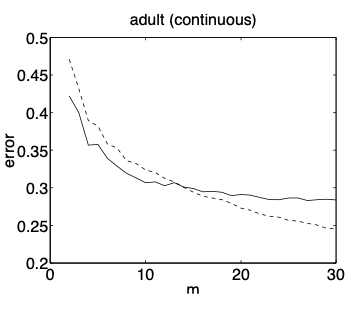
\includegraphics[scale=0.5]{figures/gen-disc}};
            \node[fill=white,inner sep=1pt] (t1) at (2.5,3) {faster convergence};
         \draw[ultra thick,red,->] (t1) -- (7,2.5);
         \node[fill=white,inner sep=1pt] (t2) at (13,4.5) {higher asymptotic error};
         \draw[ultra thick,red,->] (t2) -- (10.5,2);
\end{tikzpicture}

Solid line: naive Bayes; dashed line: logistic regression.
\end{frame}

\begin{frame}
{Naive Bayes vs logistic regression}
% \begin{table}
% \begin{tabular}{lccl}
% \toprule
% & logistic regression & GNB & \\
% \midrule
% optimization error \onslide<2->{& 0 (convex) & 0 (closed-form) &} \\
% estimation error \onslide<3->{& 0 & 0 & infinite data} \\
% approximation error \onslide<4->{& 0 & 0 & GNB assumption holds} \\
% \bottomrule
% \end{tabular}
% \end{table}
% \onslide<5->{
Logistic regression and Gaussian naive Bayes converge to the same classifier asymptotically, assuming the GNB assumption holds.

\begin{itemize}
    \item Data points are generated from Gaussian distributions for each class
    \item Each dimension is independently generated
    \item Shared variance
\end{itemize}

What if the GNB assumption is not true?

% }
% https://www.cs.princeton.edu/courses/archive/spring07/cos424/scribe_notes/0410.pdf
\end{frame}


\begin{frame}{Multivariate Gaussian Distribution}
\begin{itemize}
\item $\bx \sim {\cal N} (\mu, \Sigma)$, a Gaussian (or normal) distribution defined as
\[
p(\bx) = \frac{1}{(2 \pi)^{d/2} |\Sigma|^{1/2}} \exp \left[ -\frac{1}{2} (\bx - \mu)^T \Sigma^{-1} (\bx - \mu) \right] \
\]
% \vspace{-0.5cm}
\begin{figure}
\includegraphics[width=0.3\linewidth]{figures/gaussian2d}
\end{figure}
\onslide<2->\item Mahalanobis distance $(\bx - \mu_k)^T \Sigma^{-1} (\bx - \mu_k)$ measures the distance from $\bx$ to $\mu$ in terms of $\Sigma$
\onslide<3->\item It normalizes for difference in variances and correlations
\end{itemize}
\end{frame}

\begin{frame}{Bivariate Normal}\small
\vspace{-0.1cm}
\begin{figure}
\addtolength{\tabcolsep}{15pt}
\begin{tabular}{ccc}
$\quad$$\Sigma = \begin{pmatrix}1 & 0\\0 & 1\end{pmatrix}$ & $\ \ $ $\Sigma = 0.5\begin{pmatrix}1 & 0\\0 & 1\end{pmatrix}$ & $\Sigma = 2\begin{pmatrix}1 & 0\\0 & 1\end{pmatrix}$\\
\end{tabular}

\vspace{2.0mm}

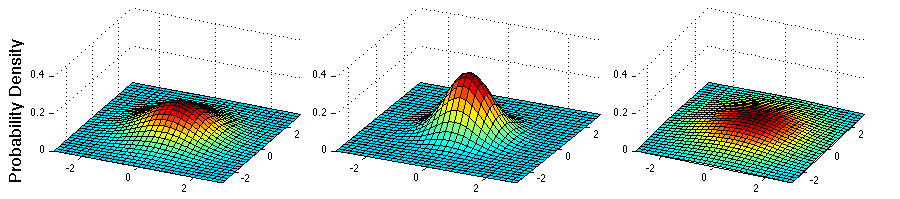
\includegraphics[width=0.8\linewidth]{figures/gauss_diag1}\\[-2.5mm]
% \caption{Probability density function}
\end{figure}
\vspace{-2.5mm}
\begin{figure}
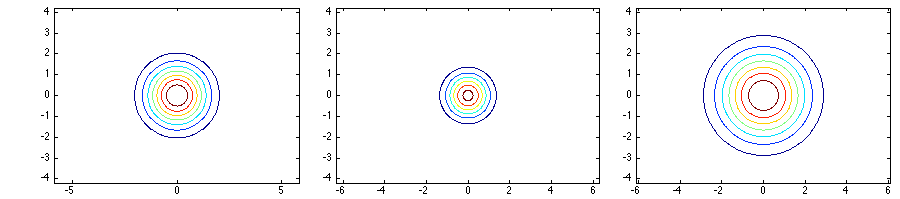
\includegraphics[width=0.8\linewidth]{figures/gauss_diag_cntr}\\[-2.5mm]
% \caption{Contour plot of the pdf}
\end{figure}
\end{frame}

\begin{frame}{Bivariate Normal}
\vspace{-0.1cm}
\begin{figure}
\addtolength{\tabcolsep}{12pt}
\begin{tabular}{ccc}
$\quad$$var(x_1)=var(x_2)$ & $var(x_1)>var(x_2)$  & $var(x_1)<var(x_2)$ \\
\end{tabular}


\vspace{2.0mm}

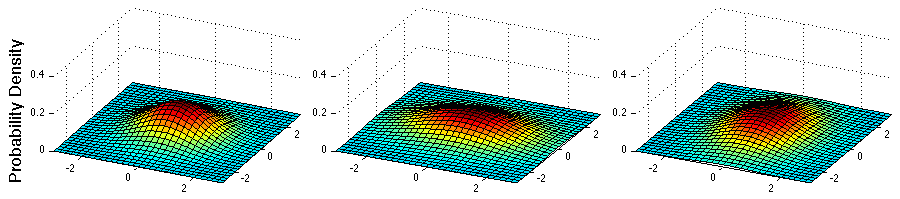
\includegraphics[width=0.8\linewidth]{figures/gauss_elongated}\\[-2.5mm]
% \caption{Probability density function}
\end{figure}
\vspace{-2.5mm}
\begin{figure}
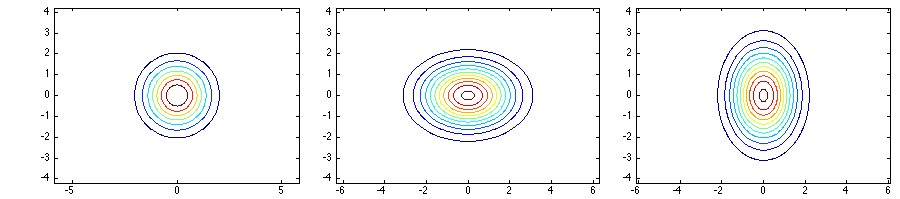
\includegraphics[width=0.8\linewidth]{figures/gauss_elongated_cntr}\\[-2.5mm]
% \caption{Contour plot of the pdf}
\end{figure}
\vspace{-0.3cm}
%\raquel{this looks wrong!}
\end{frame}

\begin{frame}{Bivariate Normal}
\vspace{-0.4cm}
\begin{figure}
\addtolength{\tabcolsep}{15pt}
\begin{tabular}{ccc}
$\quad$$\Sigma = \begin{pmatrix}1 & 0\\0 & 1\end{pmatrix}$ & $\ \ $ $\Sigma = \begin{pmatrix}1 & 0.5\\0.5 & 1\end{pmatrix}$ & $\Sigma = \begin{pmatrix}1 & 0.8\\0.8 & 1\end{pmatrix}$\\
\end{tabular}

\vspace{2.0mm}

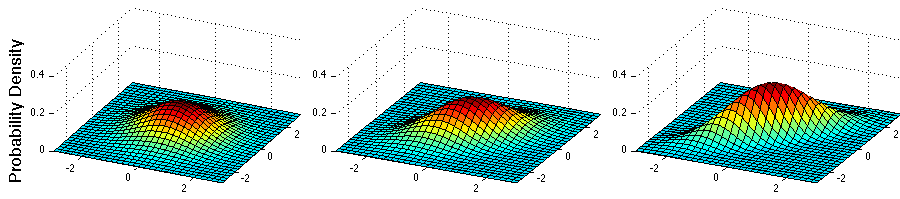
\includegraphics[width=0.8\linewidth]{figures/gauss_covpos}\\[-2.5mm]
% \caption{Probability density function}
\end{figure}
\vspace{-2.5mm}
\begin{figure}
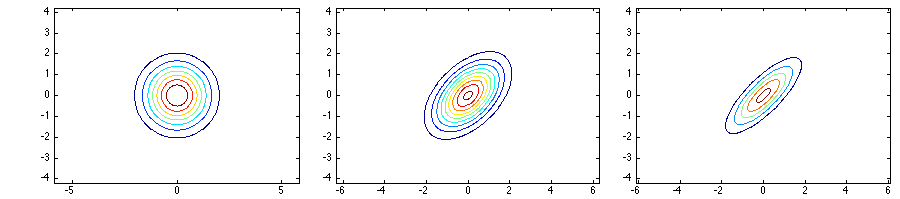
\includegraphics[width=0.8\linewidth]{figures/gauss_covpos_cntr}\\[-2.5mm]
% \caption{Contour plot of the pdf}
\end{figure}
\end{frame}

\begin{frame}{Bivariate Normal}
\vspace{-0cm}
\begin{figure}
\addtolength{\tabcolsep}{15pt}
\begin{tabular}{ccc}
$\quad$$Cov(x_1,x_2)=0$ & $Cov(x_1,x_2)>0$  & $Cov(x_1,x_2)<0$ \\
\end{tabular}

\vspace{2.0mm}

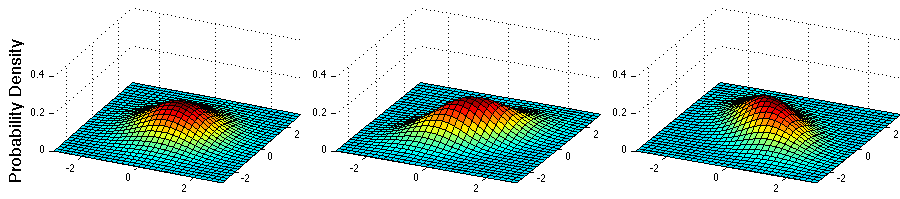
\includegraphics[width=0.8\linewidth]{figures/gauss_covneg}\\[-2.5mm]
% \caption{Probability density function}
\end{figure}
\vspace{-2.5mm}
\begin{figure}
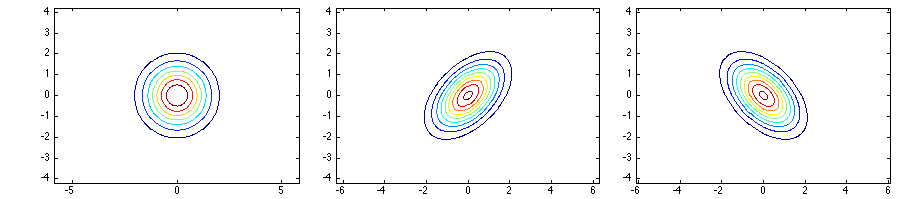
\includegraphics[width=0.8\linewidth]{figures/gauss_covneg_cntr}\\[-2.5mm]
% \caption{Contour plot of the pdf}
\end{figure}
\end{frame}

\begin{frame}{Gaussian Bayes Classifier}
\begin{itemize}
\item Gaussian Bayes Classifier in its general form assumes that $p(\bx|y)$ is distributed according to a multivariate normal (Gaussian) distribution
\item Multivariate Gaussian distribution:
\[
p(\bx|t=k) = \frac{1}{(2 \pi)^{d/2} |\Sigma_k|^{1/2}} \exp \left[ -\frac{1}{2} (\bx - \boldsymbol{\mu}_k)^T \Sigma_k^{-1} (\bx - \boldsymbol\mu_k) \right] \
\]
where $|\Sigma_k|$ denotes the determinant of the matrix, and $d$ is dimension of $\bx$
\onslide<2->\item Each class $k$ has associated mean vector $\boldsymbol{\mu}_k$ and covariance matrix $\Sigma_k$
\onslide<3->\item $\Sigma_k$ has $\mathcal{O}(d^2)$ parameters - could be hard to estimate
% (more on that later).
\end{itemize}
%\vspace{-0.5cm}
%\begin{figure}
%\includegraphics[width=0.45\linewidth]{imgs/gaussian2d}
%\end{figure}
\end{frame}


\begin{frame}{Example}
\vspace{-0.3cm}
\begin{figure}
    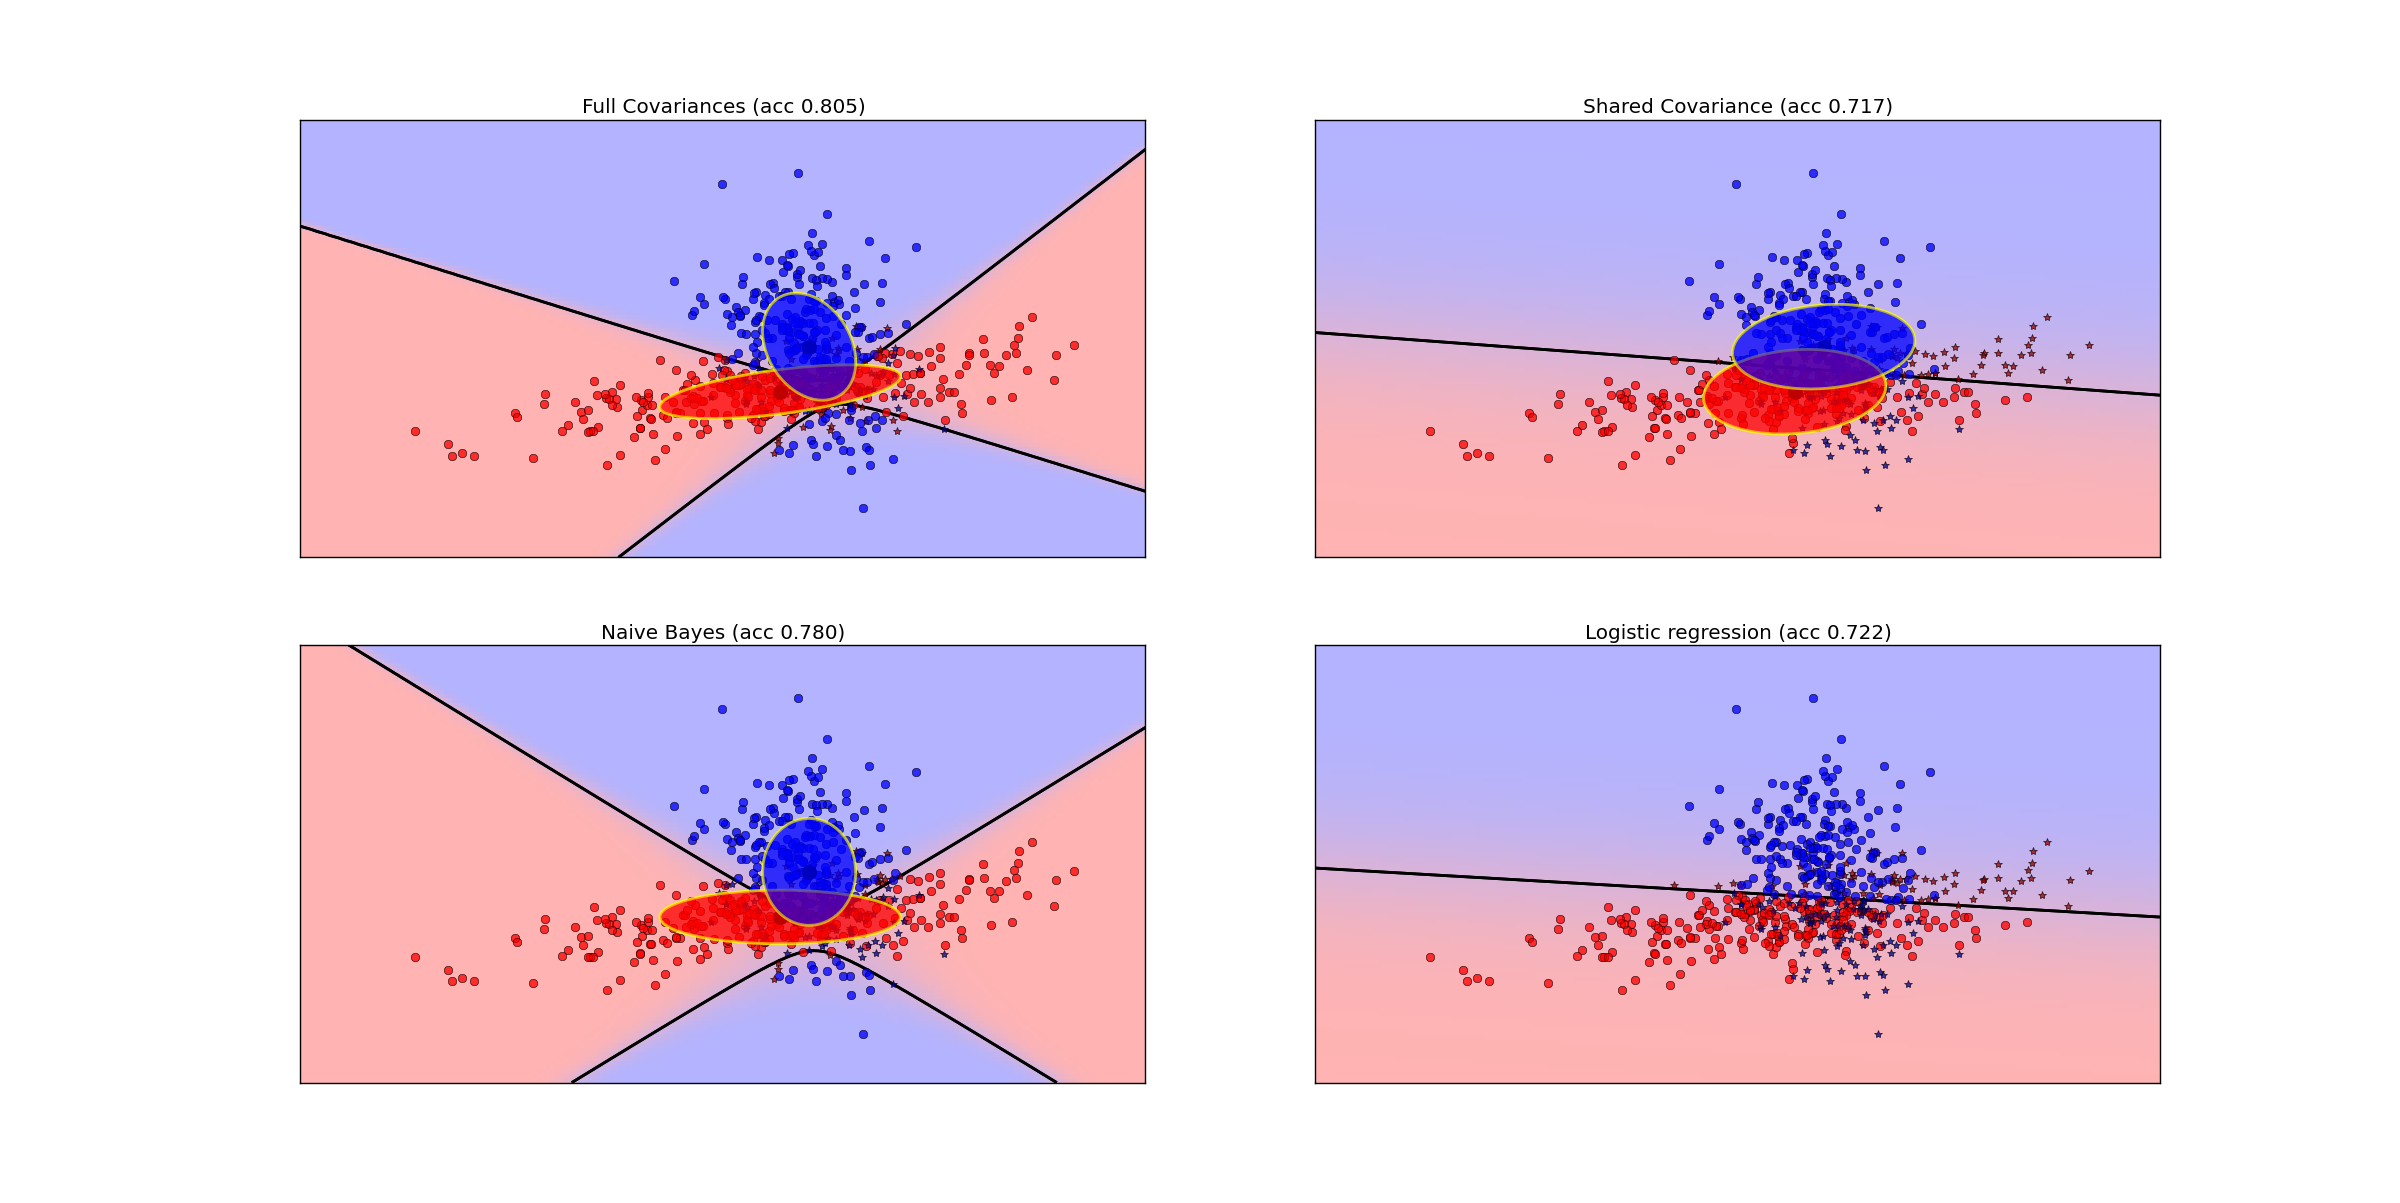
\includegraphics[width=0.8\linewidth,trim={5cm 1cm 5cm 1cm},clip]{figures/gbc_example}
\end{figure}
\end{frame}


\begin{frame}{Gaussian Bayes Binary Classifier Cases}

Different cases on the covariance matrix:
\begin{itemize}
  \item Full covariance: Quadratic decision boundary
  \item Shared covariance: Linear decision boundary
  \item Naive Bayes: Diagonal covariance matrix, quadratic decision boundary
\end{itemize}
\pause

\vspace{0.2in}

GBC vs. Logistic Regression:
\begin{itemize}
    \item If data is truly Gaussian distributed, then shared covariance = logistic regression.
    \item But logistic regression can learn other distributions.
\end{itemize}
\end{frame}

\begin{frame}{Summary}
\begin{itemize}
    \item Probabilistic framework of using maximum likelihood as a more principled way to derive loss functions.
    \item Conditional vs. generative
    \item Generative models the joint distribution, and may lead to more assumption on the data.
    \pause
    \item When there is very few data point, it may be hard to model the distribution.
    \item Is there an equivalent ``regularization'' in a probabilistic framework?
\end{itemize}
\end{frame}

\section{Bayesian ML: Classical Statistics}
\begin{frame}{Parametric Family of Densities}
\begin{itemize}
\item A \textbf{parametric family of densities }is a set 
\[
\left\{ p(y\mid\theta):\theta\in\Theta\right\} ,
\]

\begin{itemize}
\item where $p(y\mid\theta)$ is a density on a \textbf{sample space }$\cy$,
and
\item $\theta$ is a \textbf{parameter} in a {[}finite dimensional{]} \textbf{parameter
space $\Theta$.}
\end{itemize}
\end{itemize}

\pause{}
\begin{itemize}
\item This is the common starting point for a treatment of classical or
Bayesian statistics.
\item In this lecture, whenever we say ``density'', we could replace it
    with ``mass function.'' (and replace integrals with sums).{\scriptsize{} }{\scriptsize\par}
\end{itemize}
\end{frame}

\begin{frame}{Frequentist or ``Classical'' Statistics}
\begin{itemize}
\item We're still working with a parametric family of densities:
\[
\left\{ p(y\mid\theta)\mid\theta\in\Theta\right\} .
\]
\end{itemize}

\pause{}
\begin{itemize}
\item Assume that $p(y\mid\theta)$ governs the world we are observing,
for some $\theta\in\Theta$.
\end{itemize}

\pause{}
\begin{itemize}
\item If we knew the right $\theta\in\Theta$, there would be no need for
statistics.
\end{itemize}

\pause{}
\begin{itemize}
\item But instead of $\theta$, we have data $\cd$: $y_{1},\ldots,y_{n}$ sampled
i.i.d. from $p(y\mid\theta)$.
\end{itemize}

\pause{}
\begin{itemize}
\item Statistics is about how to get by with $\cd$ in place of $\theta$.
\end{itemize}
\end{frame}
%

\begin{frame}{Point Estimation}

\begin{itemize}
\item One type of statistical problem is\textbf{ point estimation}.
\end{itemize}

\pause{}
\begin{itemize}
\item A \textbf{statistic} $s=s(\cd)$ is any function of the data.
\end{itemize}

\pause{}
\begin{itemize}
\item A statistic $\hat{\theta}=\hat{\theta}(\cd)$ taking values in $\Theta$
is a\textbf{ point estimator of} $\theta$.
\end{itemize}

\pause{}
\begin{itemize}
\item A good point estimator will have $\hat{\theta}\approx\theta$.
% \end{itemize}
% \end{frame}
% %
% \begin{frame}{Desirable Properties of Point Estimators}
% \begin{itemize}
\item \textbf{Desirable statistical properties of point estimators}:

\pause{}
\begin{itemize}
\item \textbf{Consistency: }As data size $n\to\infty$, we get $\hat{\theta}_{n}\to\theta$.
\end{itemize}

\pause{}
\begin{itemize}
\item \textbf{Efficiency:} (Roughly speaking) $\hat{\theta}_{n}$ is as
accurate as we can get from a sample of size $n$.
\end{itemize}
\end{itemize}


\pause{}
\begin{itemize}
\item \textbf{Maximum likelihood estimators }are consistent and efficient
under reasonable conditions.
\end{itemize}
\end{frame}
%
% \begin{frame}{The Likelihood Function}
% \begin{itemize}
% \item Consider parametric family $\left\{ p(y\mid\theta):\theta\in\Theta\right\} $
% and i.i.d. sample $\cd=\left(y_{1},\ldots,y_{n}\right)$.

% \pause{}
% \item The density for sample $\cd$ for $\theta\in\Theta$ is
% \[
% p(\cd\mid\theta)\pause=\prod_{i=1}^{n}p(y_{i}\mid\theta).
% \]


% \pause{}
% \item $p(\cd\mid\theta)$ is a function of $\cd$ and $\theta$. 

% \pause{}
% \item For fixed $\theta$, $p(\cd\mid\theta$) is a density function on
% $\cy^{n}$.

% \pause{}
% \item For fixed $\cd$, the function $\theta\mapsto p(\cd\mid\theta)$ is
% called the \textbf{likelihood function:
% \[
% L_{\cd}(\theta):=p(\cd\mid\theta).
% \]
% }
% \end{itemize}
% \end{frame}
% %
% \begin{frame}{Maximum Likelihood Estimation}
% \begin{definition}
% The \textbf{maximum likelihood estimator (MLE)} for $\theta$ in the
% model $\left\{ p(y\mid\theta):\theta\in\Theta\right\} $ is
% \begin{eqnarray*}
% \hat{\theta}_{\text{MLE}} & = & \argmax_{\theta\in\Theta}L_{\cd}(\theta).
% \end{eqnarray*}

% \pause{}
% \end{definition}

% \begin{itemize}
% \item Maximum likelihood is just one approach to getting a point estimator
% for $\theta$.

% \pause{}
% \item \textbf{Method of moments} is another general approach one learns
% about in statistics.

% \pause{}
% \item Later we'll talk about \textbf{MAP }and \textbf{posterior mean }as
% approaches to point estimation.
% \begin{itemize}
% \item These arise naturally in Bayesian settings.
% \end{itemize}
% \end{itemize}
% \end{frame}
%
\begin{frame}{Example of Point Estimation: Coin Flipping}
\begin{itemize}
\item Parametric family of mass functions:
\[
p(\text{Heads}\mid\theta)=\theta,
\]
for $\theta\in\Theta=\left(0,1\right)$.
\end{itemize}
\end{frame}
%
\begin{frame}{Coin Flipping: MLE}
\begin{itemize}
\item Data $\cd=\left(H,H,T,T,T,T,T,H,\ldots,T\right)$, assumed i.i.d. flips.
\begin{itemize}
\item $n_{h}$: number of heads
\item $n_{t}$: number of tails\textbf{ }
\end{itemize}
% \item 

\pause{}
\item \textbf{Likelihood function }for data $\cd$:

\[
L_{\cd}(\theta)=\pause p(\cd\mid\theta)=\theta^{n_{h}}\left(1-\theta\right)^{n_{t}}
\]

% \pause{}
% \item (This is the probability of getting the flips in the order they were
% received)
% \end{itemize}
% \end{frame}
%
% \begin{frame}{Coin Flipping: MLE}
 
% \begin{itemize}
\item As usual, it is easier to maximize the log-likelihood function:
\begin{eqnarray*}
\hat{\theta}_{\text{MLE}} & = & \argmax_{\theta\in\Theta}\log L_{\cd}(\theta)\\
 & = & \argmax_{\theta\in\Theta}\left[n_{h}\log\theta+n_{t}\log(1-\theta)\right]
\end{eqnarray*}
\end{itemize}

\pause{}
\begin{itemize}
    \item First order condition (equating the derivative to zero):
\[
\frac{n_{h}}{\theta}-\frac{n_{t}}{1-\theta} = 0 \iff\theta  =  \frac{n_{h}}{n_{h}+n_{t}} \pause \quad \quad  \hat{\theta}_{\text{MLE}} \text{ is the empirical fraction of heads.}
\]
% \item So $\hat{\theta}_{\text{MLE}}$ 
\end{itemize}
\end{frame}

\section{Bayesian Statistics: Introduction}
\begin{frame}{Bayesian Statistics}
 

\begin{itemize}
\item Baysian statistics introduces a crucial new ingredient: the \textbf{prior distribution.}
\end{itemize}

\pause{}
\begin{itemize}
\item A \textbf{prior distribution} $p(\theta)$ is a distribution on the parameter
space $\Theta$.
\end{itemize}

\pause{}
\begin{itemize}
\item The prior reflects our belief about $\theta$, \textbf{before seeing
any data}.
\end{itemize}
\end{frame}
%
\begin{frame}{A Bayesian Model }
\begin{itemize}
\item A {[}parametric{]} Bayesian model consists of two pieces:
\begin{enumerate}
\item A parametric family of densities 
\[
\left\{ p(\cd\mid\theta)\mid\theta\in\Theta\right\} .
\]


\pause{}
\item A \textbf{prior distribution} $p(\theta)$ on parameter space $\Theta$.

\pause{}
\end{enumerate}
\item Putting the pieces together, we get a joint density on $\theta$ and $\cd$:
\[
p(\cd,\theta)=p(\cd\mid\theta)p(\theta).
\]
\end{itemize}
\end{frame}
%
\begin{frame}{The Posterior Distribution}
\begin{itemize}
\item The \textbf{posterior distribution }for $\theta$ is $p(\theta\mid\cd)$.
\end{itemize}

\pause{}
\begin{itemize}
\item Whereas the prior represents belief about $\theta$ before observing data $\cd$,
\end{itemize}

\pause{}
\begin{itemize}
\item The posterior represents the\textbf{ rationally updated belief}
about $\theta$, after seeing $\cd$.
\end{itemize}
\end{frame}
%
\begin{frame}{Expressing the Posterior Distribution}
\begin{itemize}
\item By Bayes rule, can write the posterior distribution as
\[
p(\theta\mid\cd)\pause=\frac{p(\cd\mid\theta)p(\theta)}{p(\cd)}.
\]


\pause{}
\item Let's consider both sides as functions of $\theta$, for fixed $\cd$.

\pause{}
\item Then both sides are densities on $\Theta$ and we can write
\[
\underbrace{p(\theta\mid\cd)}_{\text{posterior}}\propto\underbrace{p(\cd\mid\theta)}_{\text{likelihood}}\underbrace{p(\theta)}_{\text{prior}}.
\]


\pause{}
\item Where $\propto$ means we've dropped factors that are independent of $\theta$. 
\end{itemize}
\end{frame}
%
\begin{frame}{Coin Flipping: Bayesian Model}
\begin{itemize}
\item Recall that we have a parametric family of mass functions:
\[
p(\text{Heads}\mid\theta)=\theta,
\]
for $\theta\in\Theta=\left(0,1\right)$.
\end{itemize}

\pause{}
\begin{itemize}
\item We need a prior distribution $p(\theta)$ on $\Theta=(0,1)$.
\end{itemize}

\pause{}
\begin{itemize}
\item One convenient choice would be a distribution from the Beta family
\end{itemize}
\end{frame}
%
\begin{frame}{Coin Flipping: Beta Prior}
\begin{itemize}
\item \textbf{Prior:}
\begin{eqnarray*}
\theta & \sim & \text{Beta}(\alpha,\beta)\\
p(\theta) & \propto & \theta^{\alpha-1}\left(1-\theta\right)^{\beta-1}
\end{eqnarray*}


\pause{}
\end{itemize}
\begin{center}
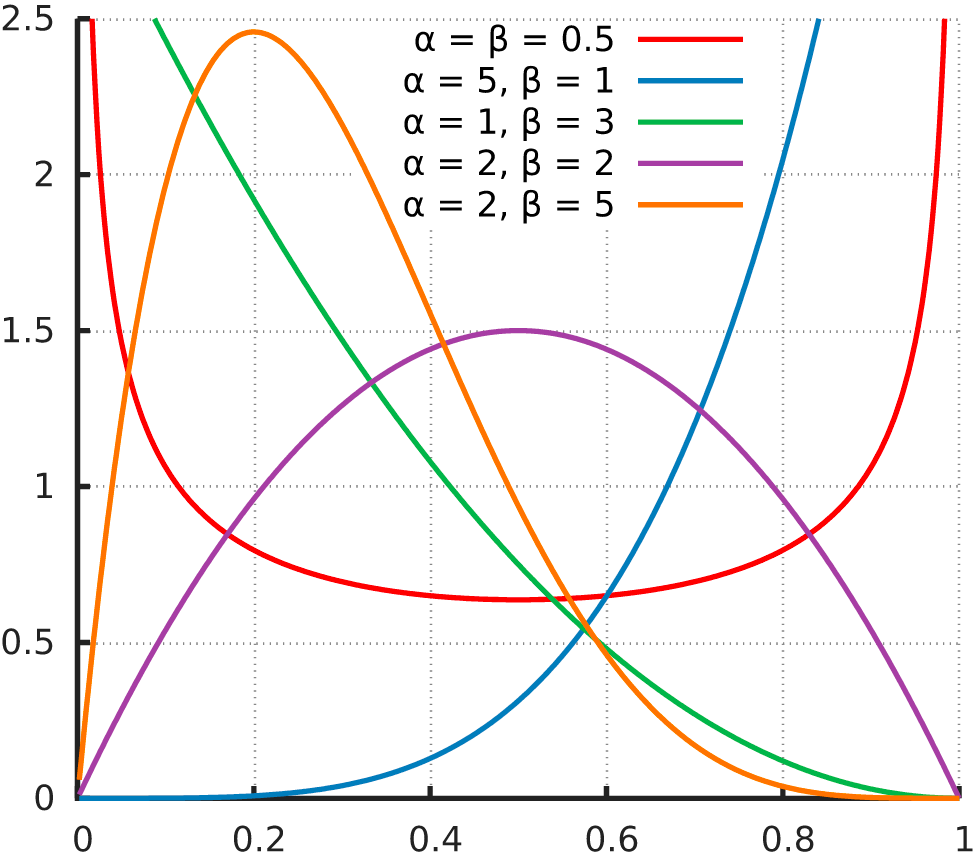
\includegraphics[height=0.55\textheight]{figures/betaFamily}
\par\end{center}


\let\thefootnote\relax\footnotetext{\tiny{Figure by Horas based on the work of Krishnavedala (Own work) [Public domain], via Wikimedia Commons \url{http://commons.wikimedia.org/wiki/File:Beta_distribution_pdf.svg}.}}
\end{frame}

%
\begin{frame}{Coin Flipping: Beta Prior}
\begin{itemize}
\item \textbf{Prior:}
\begin{eqnarray*}
\theta & \sim & \text{Beta}(h,t)\\
p(\theta) & \propto & \theta^{h-1}\left(1-\theta\right)^{t-1}
\end{eqnarray*}


\pause{}
\item \textbf{Mean of Beta distribution:} 
\[
\ex\theta=\frac{h}{h+t}
\]


\pause{}
\item \textbf{Mode of Beta distribution:} 
\[
\argmax_{\theta}p(\theta)=\frac{h-1}{h+t-2}
\]
for $h,t>1$.
\end{itemize}
\end{frame}
%
\begin{frame}{Coin Flipping: Posterior}
\begin{itemize}
\item \textbf{Prior:}
\begin{eqnarray*}
\theta & \sim & \text{Beta}(h,t)\\
p(\theta) & \propto & \theta^{h-1}\left(1-\theta\right)^{t-1}
\end{eqnarray*}
\end{itemize}

\pause{}
\begin{itemize}
\item \textbf{Likelihood function}
\[
L(\theta)=p(\cd\mid\theta)=\theta^{n_{h}}\left(1-\theta\right)^{n_{t}}
\]
\end{itemize}

\pause{}
\begin{itemize}
\item \textbf{Posterior density:}
\begin{eqnarray*}
p(\theta\mid\cd) & \propto & p(\theta)p(\cd\mid\theta)\\
\pause & \propto & \theta^{h-1}\left(1-\theta\right)^{t-1}\times\theta^{n_{h}}\left(1-\theta\right)^{n_{t}}\\
\pause & = & \theta^{h-1+n_{h}}\left(1-\theta\right)^{t-1+n_{t}}
\end{eqnarray*}
 
\end{itemize}
\end{frame}
%
\begin{frame}{The Posterior is in the Beta Family!}
\begin{itemize}
\item \textbf{Prior:}
\begin{eqnarray*}
\theta & \sim & \text{Beta}(h,t)\\
p(\theta) & \propto & \theta^{h-1}\left(1-\theta\right)^{t-1}
\end{eqnarray*}
 
\item \textbf{Posterior density:}
\begin{eqnarray*}
p(\theta\mid\cd) & \propto & \theta^{h-1+n_{h}}\left(1-\theta\right)^{t-1+n_{t}}
\end{eqnarray*}
\end{itemize}

\pause{}
\begin{itemize}
\item \textbf{Posterior is in the beta family}:
\begin{eqnarray*}
\theta\mid\cd & \sim & \text{Beta}(h+n_{h},t+n_{t})
\end{eqnarray*}
\end{itemize}

\pause{}
\begin{itemize}
\item \textbf{Interpretation}:
\begin{itemize}
\item Prior initializes our counts with $h$ heads and $t$ tails.
\item Posterior increments counts by observed $n_{h}$ and $n_{t}$. 
\end{itemize}
\end{itemize}
\end{frame}
%
\begin{frame}{Sidebar: Conjugate Priors}
\begin{itemize}
\item In this case, the posterior is in the same distribution family as the prior.
\item Let $\pi$ be a family of prior distributions on $\Theta$.

\pause{}
\item Let $P$ parametric family of distributions with parameter space $\Theta$.

\pause{}

\end{itemize}
\begin{definition}
A family of distributions \textbf{$\pi$ is conjugate to }parametric
model \textbf{$P$} if for any prior in $\pi$, the posterior is always
in $\pi$.

\pause{}
\end{definition}

\begin{itemize}
\item The beta family is conjugate to the coin-flipping (i.e. Bernoulli)
model.

%\pause{}
%\item The family of all probability distributions is conjugate to any parametric
%model. {[}Trvially{]}
\end{itemize}

\end{frame}
%
\begin{frame}{Coin Flipping: Concrete Example}
\begin{itemize}
\item Suppose we have a coin, possibly biased (\textbf{parametric probability
model}):
\[
p(\mbox{Heads}\mid\theta)=\theta.
\]


\pause{}
\item \textbf{Parameter space }$\theta\in\Theta=[0,1]$. 
\item \textbf{Prior distribution: }$\theta\sim\mbox{Beta}(2,2)$.

\pause{}
\end{itemize}
\begin{center}
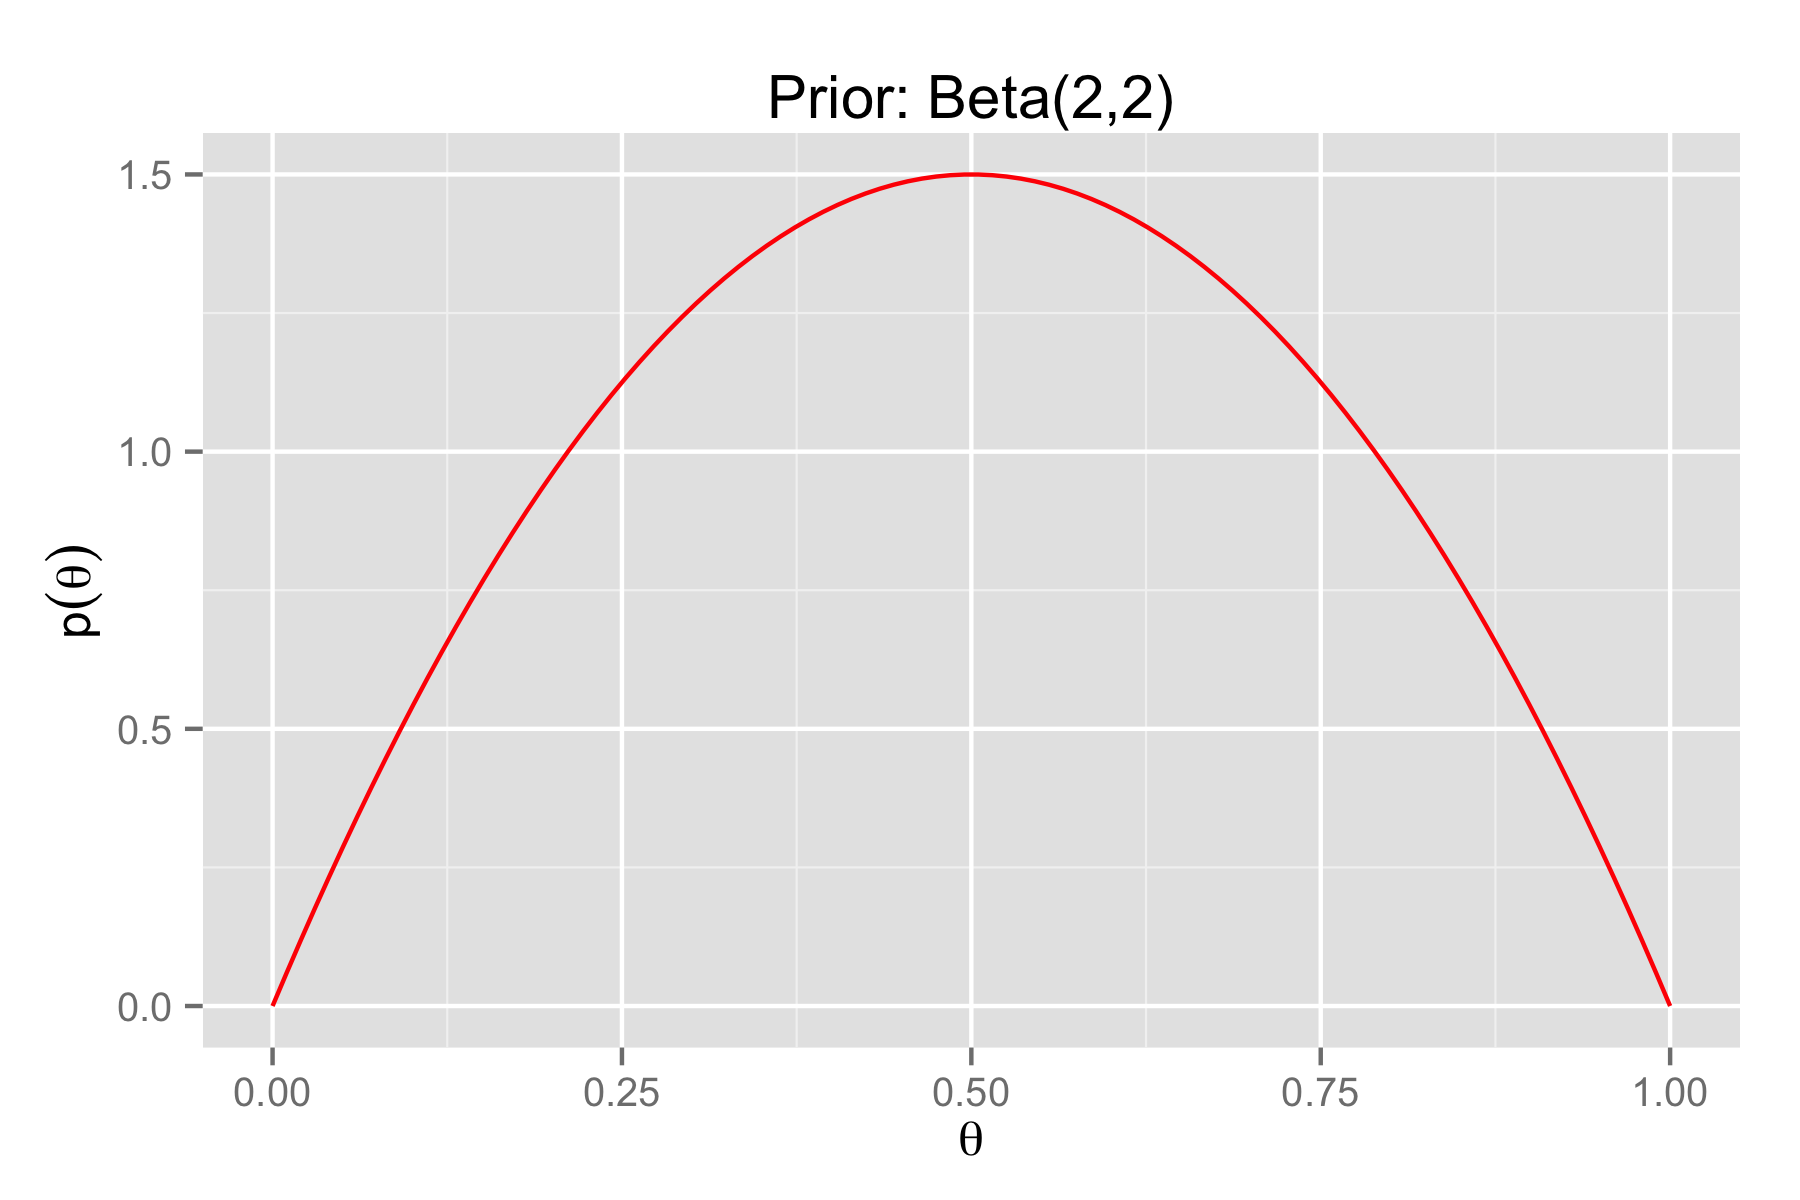
\includegraphics[height=0.5\textheight]{figures/beta2-2}
\par\end{center}

\end{frame}
%
\begin{frame}{Example: Coin Flipping}
\begin{itemize}
\item Next, we gather some data $\cd=\left\{ H,H,T,T,T,T,T,H,\ldots,T\right\} $:
\end{itemize}

\pause{}
\begin{itemize}
\item Heads: 75\qquad{}Tails: 60 

\pause{}
\begin{itemize}
\item $\hat{\theta}_{\text{MLE}}=\frac{75}{75+60}\approx0.556$

\pause{}
\end{itemize}
\item \textbf{Posterior distribution: $\theta\mid\cd\sim\mbox{Beta}(77,62)$:}
\end{itemize}
\begin{center}
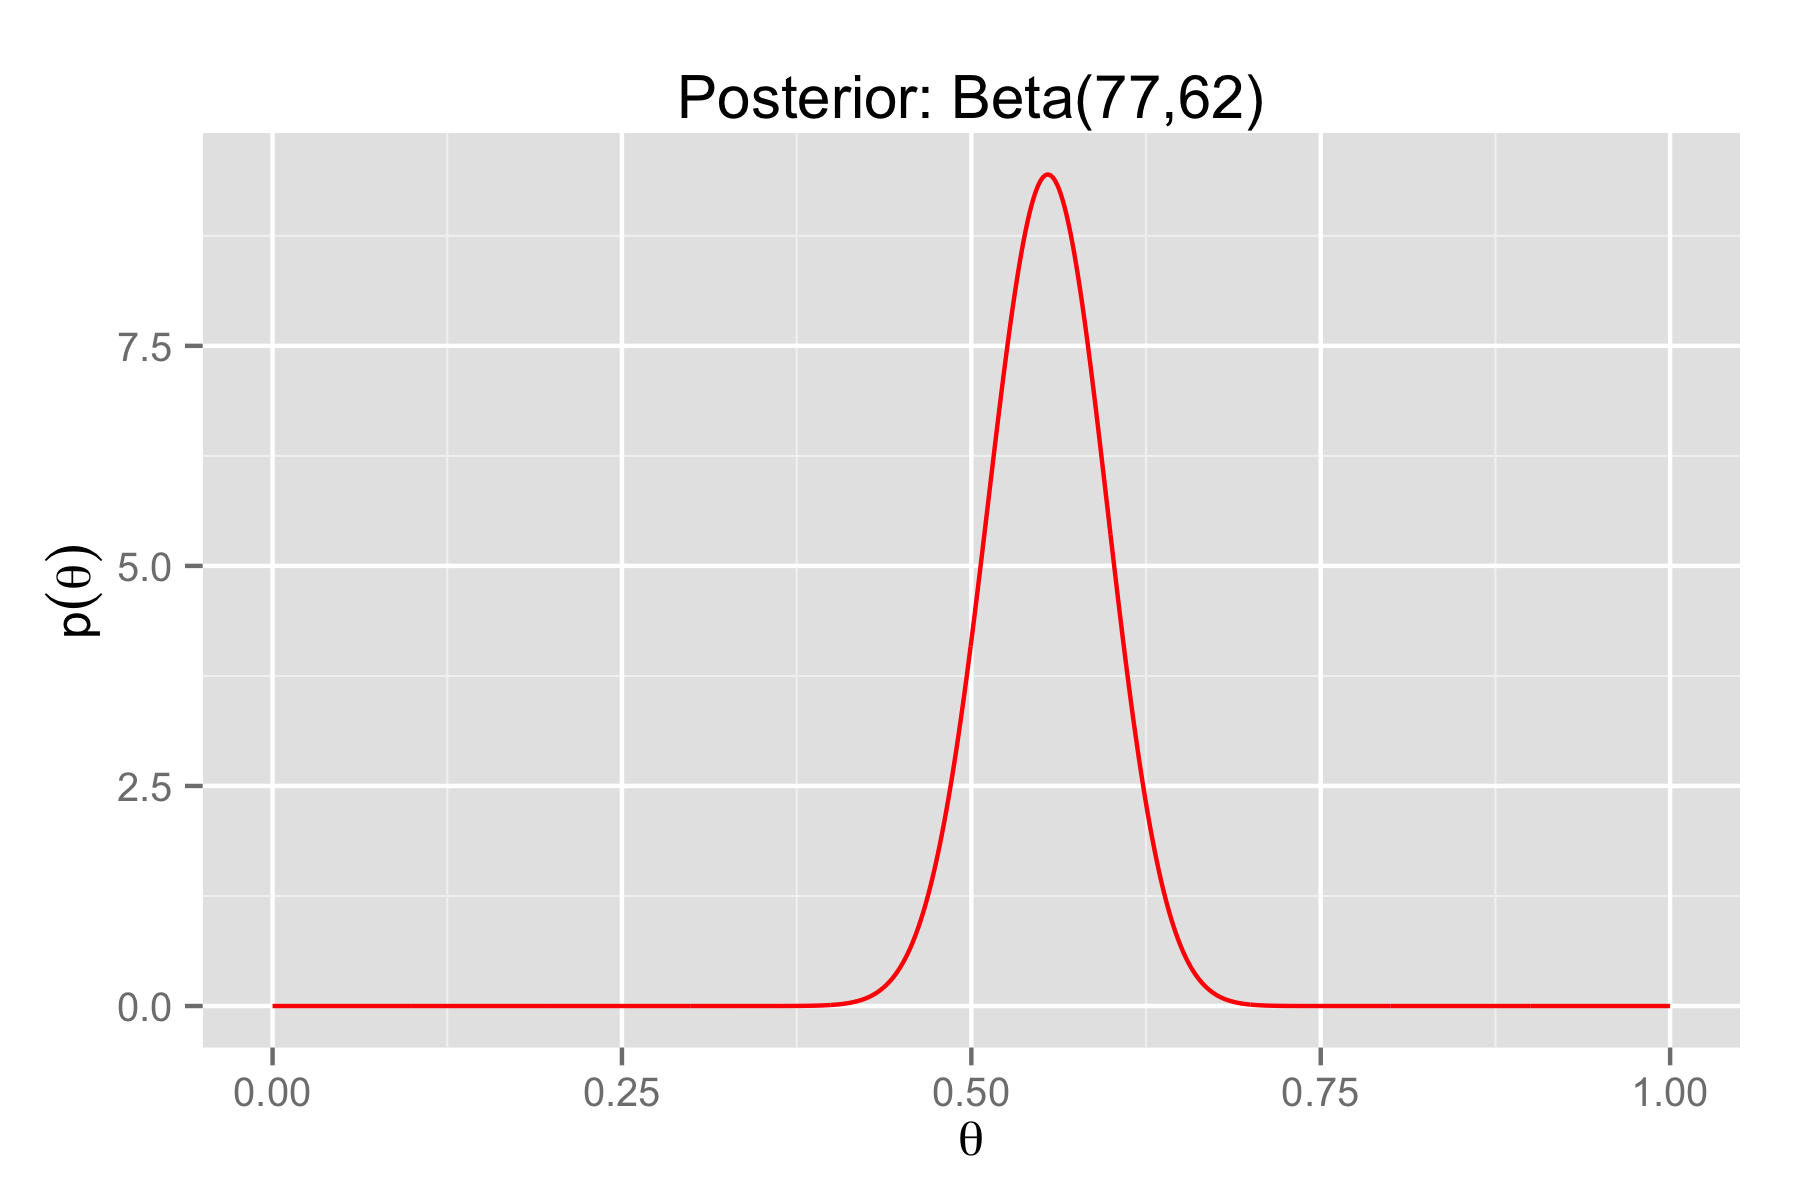
\includegraphics[height=0.6\textheight]{figures/beta77-62}
\par\end{center}

\end{frame}

\begin{frame}{Bayesian Point Estimates}
\begin{itemize}
\item We have the posterior distribution $\theta\mid\cd$.
\item What if someone asks us for a point estimate $\hat{\theta}$ for $\theta$?

\pause{}
\item Common options:

\pause{}
\begin{itemize}
\item \textbf{posterior mean} $\hat{\theta}=\ex\left[\theta\mid\cd\right]$

\pause{}
\item \textbf{maximum a posteriori (MAP) estimate} $\hat{\theta}=\argmax_{\theta}p(\theta\mid\cd)$ 
\begin{itemize}
\item Note: this is the \textbf{mode} of the posterior distribution
\end{itemize}
\end{itemize}
\end{itemize}
\end{frame}
%
\begin{frame}{What else can we do with a posterior?}
\begin{itemize}
\item Look at it: display uncertainty estimates to our client

\pause{}
\item Extract a \textbf{credible set} for $\theta$ (a Bayesian confidence
interval).
\begin{itemize}
\item e.g. Interval $[a,b]$ is a $95\%$\textbf{ credible set} if\textbf{
\[
\pr\left(\theta\in[a,b]\mid\cd\right)\ge0.95
\]
 }
\end{itemize}

\pause{}
\item Select a point estimate using \textbf{Bayesian decision theory}:
\begin{itemize}
\item Choose a loss function.
\item Find action \textbf{minimizing expected risk w.r.t. posterior}
\end{itemize}
\end{itemize}

\end{frame}

\section{Bayesian Decision Theory}
\begin{frame}{Bayesian Decision Theory}
\begin{itemize}
\item Ingredients: 
\begin{itemize}
\item \textbf{Parameter space} $\Theta$.
\item \textbf{Prior}: Distribution $p(\theta)$ on $\Theta$.
\item \textbf{Action space} $\ca$.
\item \textbf{Loss function}: $\ell:\ca\times\Theta\to\reals$.

\pause{}
\end{itemize}
\item The \textbf{posterior risk} of an action $a\in\ca$ is 
\begin{eqnarray*}
r(a) & := & \ex\left[\ell(\theta,a)\mid\cd\right]\\
\pause & = & \int\ell(\theta,a)p(\theta\mid\cd)\,d\theta.
\end{eqnarray*}


\pause{}
\begin{itemize}
\item It's the \textbf{expected loss under the posterior.}

\pause{}
\end{itemize}
\item A \textbf{Bayes action} $a^{*}$ is an action that minimizes posterior
risk:
\[
r(a^{*})=\min_{a\in\ca}r(a)
\]
\end{itemize}
\end{frame}
%
\begin{frame}{Bayesian Point Estimation}
\begin{itemize}
\item General Setup:
\begin{itemize}
\item Data $\cd$ generated by $p(y\mid\theta)$, for unknown $\theta\in\Theta$.

\pause{}
\item We want to produce a \textbf{point estimate} for $\theta$.

\pause{}
\end{itemize}
\item Choose:

\pause{}
\begin{itemize}
\item \textbf{Prior} $p(\theta)$ on $\Theta=\reals$.

\pause{}
\item \textbf{Loss} $\ell(\hat{\theta},\theta)$ %=\left(\theta-\hat{\theta}\right)^{2}$ 

\pause{}
\end{itemize}
\item Find \textbf{action} $\hat{\theta}\in\Theta$ that minimizes the \textbf{
posterior risk:}
\begin{eqnarray*}
r(\hat{\theta}) & = & \ex\left[\ell(\hat{\theta},\theta)\mid\cd\right]\\
\pause & = & \int\ell(\hat{\theta},\theta)p(\theta\mid\cd)\,d\theta
\end{eqnarray*}
\end{itemize}
\end{frame}
%
\begin{frame}{Important Cases}
\begin{itemize}
  \item Squared Loss :  $\ell(\hat{\theta},\theta)=\left(\theta-\hat{\theta}\right)^{2} \quad \Rightarrow$ posterior mean
  \item Zero-one Loss:  $\ell(\theta,\hat{\theta})=\ind{\theta\neq\hat{\theta}}\quad \Rightarrow $ posterior mode
  \item Absolute Loss :  $\ell(\hat{\theta},\theta)=\left|\theta-\hat{\theta}\right| \quad \Rightarrow$ posterior median
\end{itemize}
\end{frame}
%
\begin{frame}{Bayesian Point Estimation: Square Loss}
\begin{itemize}
\item Find \textbf{action} $\hat{\theta}\in\Theta$ that minimizes\textbf{
posterior risk} 
\begin{eqnarray*}
r(\hat{\theta}) & = & \int\left(\theta-\hat{\theta}\right)^{2}p(\theta\mid\cd)\,d\theta.
\end{eqnarray*}


\pause{}
\item Differentiate:
\end{itemize}
\begin{eqnarray*}
\frac{dr(\hat{\theta})}{d\hat{\theta}} & = & -\int2\left(\theta-\hat{\theta}\right)p(\theta\mid\cd)\,d\theta\\
\pause & = & -2\int\theta p(\theta\mid\cd)\,d\theta+2\hat{\theta}\underbrace{\int p(\theta\mid\cd)\,d\theta}_{=1}\\
\pause & = & -2\int\theta p(\theta\mid\cd)\,d\theta+2\hat{\theta}
\end{eqnarray*}

\end{frame}
%
\begin{frame}{Bayesian Point Estimation: Square Loss}
\begin{itemize}
\item Derivative of posterior risk is
\[
\frac{dr(\hat{\theta})}{d\hat{\theta}}=-2\int\theta p(\theta\mid\cd)\,d\theta+2\hat{\theta}.
\]


\pause{}
\item First order condition $\frac{dr(\hat{\theta})}{d\hat{\theta}}=0$
gives
\begin{eqnarray*}
\hat{\theta} & = & \int\theta p(\theta\mid\cd)\,d\theta\\
\pause & = & \ex\left[\theta\mid\cd\right]
\end{eqnarray*}
\end{itemize}

\pause{}
\begin{itemize}
\item The \textbf{Bayes action }for \textbf{square loss} is the posterior mean.
\end{itemize}
\end{frame}
%
% \begin{frame}{Bayesian Point Estimation: Absolute Loss}
% \begin{itemize}
% \item \textbf{Loss:}\emph{ $\ell(\theta,\hat{\theta})=\left|\theta-\hat{\theta}\right|$}

% \pause{}
% \item \textbf{Bayes action} for \textbf{absolute loss} is the \textbf{posterior
% median.}
% \begin{itemize}
% \item That is, the median of the distribution $p(\theta\mid\cd)$.

% \pause{}
% \item Show with approach similar to what was used in Homework \#1.
% \end{itemize}
% \end{itemize}
% \end{frame}
%
%\begin{frame}{Bayesian Point Estimation: Zero-One Loss}
%\begin{itemize}
%\item Suppose $\Theta$ is discrete (e.g. $\Theta=\left\{ \mbox{english},\mbox{french}\right\} $)
%\item \textbf{Zero-one loss:}\emph{ $\ell(\theta,\hat{\theta})=\ind{\theta\neq\hat{\theta}}$}

%\pause{}
%\item \textbf{Posterior risk}:
%\begin{eqnarray*}
%r(\hat{\theta}) & = & \ex\left[\ind{\theta\neq\hat{\theta}}\mid\cd\right]\\
%\pause & = & \pr\left(\theta\neq\hat{\theta}\mid\cd\right)\\
%\pause & = & 1-\pr\left(\theta=\hat{\theta}\mid\cd\right)\\
%\pause & = & 1-p(\hat{\theta}\mid\cd)
%\end{eqnarray*}


%\pause{}
%\item \textbf{Bayes action} is
%\begin{eqnarray*}
%\hat{\theta} & = & \argmax_{\theta\in\Theta}p(\theta\mid\cd)
%\end{eqnarray*}


%\pause{}
%\item This $\hat{\theta}$ is called the\textbf{ maximum a posteriori (MAP)
%}estimate.
%\item The MAP estimate is the \textbf{mode} of the posterior distribution.
%\end{itemize}
%\end{frame}

\section{Interim summary}
\begin{frame}{Recap and Interpretation}
\begin{itemize}
\item The prior represents belief about $\theta$ before observing data $\cd$.
\item The posterior represents \textbf{ rationally updated beliefs}
after seeing $\cd$.

\pause{}
\item All inferences and action-taking are based on the posterior distribution.

\pause{}
\item In the Bayesian approach,
\begin{itemize}
\item No issue of justifying an estimator.

\pause{}
\item Only choices are
\begin{itemize}
\item \textbf{family of distributions}, indexed by $\Theta$, and
\item \textbf{prior distribution }on $\Theta$

\pause{}
\end{itemize}
\item For decision making, we need a \textbf{loss function}.
\end{itemize}
\end{itemize}
\emph{}
\end{frame}
%
%\begin{frame}{The Bayesian Method}
 
%\begin{enumerate}
%\item \textbf{Define the model}:
%\begin{itemize}
%\item Choose a parametric family of densities: 
%\[
%\left\{ p(\cd\mid\theta)\mid\theta\in\Theta\right\} .
%\]
 
%\item Choose a distribution $p(\theta)$ on $\Theta$, called the \textbf{prior
%distribution}.

%\pause{}
%\end{itemize}
%\item After observing $\cd$, compute the \textbf{posterior distribution}
%$p(\theta\mid\cd)$. 

%\pause{}
%\item Choose  \textbf{action} based on $p(\theta\mid\cd)$. 
%\end{enumerate}
%\end{frame}
%

\section{Recap: Conditional Probability Models}
\begin{frame}{Conditional Probability Modeling}

\begin{itemize}
\item \textbf{Input space} $\cx$
\item \textbf{Outcome space} $\cy$ 

% \pause{}
\item \textbf{Action space} $\ca=\left\{ p(y)\mid p\text{ is a probability distribution on }\cy\right\} $.

\pause{}
\item \textbf{Hypothesis space} $\cf$ contains prediction functions $f:\cx\to\ca$. 

% \pause{}
\item \textbf{Prediction function} $f\in\cf$ takes input $x\in\cx$ and
produces a \textbf{distribution} on $\cy$

\pause{}
% \item We've been discussing \textbf{parametric families of conditional densities}
% \[
% \left\{ p(y\mid x,\theta):\theta\in\Theta\right\} .
% \]


% \pause{}
% \item These are also hypothesis spaces for conditional probability modeling.

% \pause{}
% \item Examples?
% \end{itemize}
% \end{frame}
% %
% \begin{frame}{Parametric Family of Conditional Densities}
% \begin{itemize}
\item A \textbf{parametric family of conditional densities }is a set 
\[
\left\{ p(y\mid x,\theta):\theta\in\Theta\right\} ,
\]

\begin{itemize}
\item where $p(y\mid x,\theta)$ is a density on \textbf{outcome space }$\cy$
for each $x$ in \textbf{input space $\cx$}, and
\item $\theta$ is a \textbf{parameter} in a {[}finite dimensional{]} \textbf{parameter
space $\Theta$.}
\end{itemize}
\end{itemize}

\pause{}
\begin{itemize}
\item This is the common starting point for either classical or
Bayesian regression.
\end{itemize}
\end{frame}
%
% \begin{frame}{Density vs Mass Functions}
% \begin{itemize}
% \item In this lecture, whenever we say ``density'', we could replace it
% with ``mass function.'' 
% \end{itemize}

% \pause{}
% \begin{itemize}
% \item Corresponding integrals would be replaced by summations.{\scriptsize{} }{\scriptsize\par}
% \end{itemize}

% \pause{}
% \begin{itemize}
% \item {\small{}(In more advanced, measure-theoretic treatments, they are
% each considered densities w.r.t. different base measures.)}{\small\par}
% \end{itemize}
% \end{frame}
%
% \begin{frame}{The Data: Assumptions So Far in this Course}
% \begin{itemize}
% \item Our usual setup is that $(x,y)$ pairs are drawn i.i.d. from $\cp_{\cx\times\cy}$.

% \pause{}
% \item How have we used this assumption so far?

% \pause{}
% \begin{itemize}
% \item ties validation performance to test performance
% \item ties test performance to performance on new data when deployed
% \item motivates empirical risk minimization

% \pause{}
% \end{itemize}
% \item The large majority of things we've learned about ridge/lasso/elastic-net
% regression, optimization, SVMs, and kernel methods are true for arbitrary
% training data sets $\cd:\left(x_{1},y_{1}\right),\ldots,\left(x_{n},y_{n}\right)\in\cx\times\cy$.
% \begin{itemize}
% \item i.e. $\cd$ could be created by hand, by an adversary, or randomly.

% \pause{}
% \end{itemize}
% \item We rely on the i.i.d. $\cp_{\cx\times\cy}$ assumption when it comes
% to \textbf{generalization}.
% \end{itemize}
% \end{frame}
% %
% \begin{frame}{The Data: Conditional Probability Modeling}
% \begin{itemize}
% \item To get generalization, we'll still need our usual i.i.d. $\cp_{\cx\times\cy}$
% assumption.
% \end{itemize}

% \pause{}
% \begin{itemize}
% \item For developing the model, we'll make some assumptions about the training
% data...
% \begin{itemize}
% \item In most of what we've done before, we had no assumptions on the training
% data.
% \end{itemize}
% \end{itemize}

% \pause{}
% \begin{itemize}
% \item It's typical (and most general) to do everything ``conditional on
% the $x$'s''
% \begin{itemize}
% \item That means, we assume the $x$'s are known

% \pause{}
% \item In particular, we do not consider them random

% \pause{}
% \item We don't care how they were generated (randomly, adversarially, chosen
% by hand) 

% \pause{}
% \item In other words, still no assumptions on $x$'s. 
% \end{itemize}
% \end{itemize}
% \end{frame}
% %
% \begin{frame}{The Data: Conditional Probability Modeling}
% \begin{itemize}
% \item So we assume the $x$'s are known.
% \end{itemize}

% \pause{}
% \begin{itemize}
% \item We observe $y_{i}$ sampled randomly from $p(y\mid x_{i},\theta)$,
% for some unknown $\theta\in\Theta$. 
% \end{itemize}

% \pause{}
% \begin{itemize}
% \item We assume the outcomes $y_{1},\ldots,y_{n}$ are independent. 
% \begin{itemize}
% \item But not i.i.d. -- Why?
% \end{itemize}

% \pause{}
% \begin{itemize}
% \item Each $y_{i}$ may be drawn from a different distribution, depending
% on $x_{i}$.
% \end{itemize}

% \end{itemize}
% \end{frame}
%
\begin{frame}{Classical treatment: Likelihood Function}
\begin{itemize}
\item \textbf{Data: }$\cd=(y_{1},\ldots,,y_{n})$
\item The probability density for our data $\cd$ is
\begin{eqnarray*}
p(\cd\mid x_{1},\ldots,x_{n},\theta) & = & \prod_{i=1}^{n}p(y_{i}\mid x_{i},\theta).
\end{eqnarray*}


\pause{}
\item For fixed $\cd$, the function $\theta\mapsto p(\cd\mid x,\theta)$
is the \textbf{likelihood function}:
\[
L_{\cd}(\theta)=p(\cd\mid x,\theta),
\]
where $x=\left(x_{1},\ldots,x_{n}\right)$.
\end{itemize}
\end{frame}
%
\begin{frame}{Maximum Likelihood Estimator}
\begin{itemize}
\item The \textbf{maximum likelihood estimator (MLE)} for $\theta$ in the
family $\left\{ p(y\mid x,\theta)\mid\theta\in\Theta\right\} $ is
\begin{eqnarray*}
\hat{\theta}_{\text{MLE}} & = & \argmax_{\theta\in\Theta}L_{\cd}(\theta).
\end{eqnarray*}


% \pause{}
\item MLE corresponds to ERM, if we set the loss to be the negative log-likelihood.

\pause{}
\item The corresponding prediction function is
\[
\hat{f}(x)=p(y\mid x,\hat{\theta}_{\text{MLE}}).
\]


%\pause{}
%\item We can think of this as a choice of a particular function from the
%hypothesis space
%\[
%\cf=\left\{ p(y\mid x,\theta):\theta\in\Theta\right\} .
%\]
\end{itemize}
\end{frame}

\section{Bayesian Conditional Probability Models}
\begin{frame}{Bayesian Conditional Models}
\begin{itemize}
\item Input space $\cx=\reals^{d}$\qquad{}Outcome space $\cy=\reals$
\end{itemize}

\pause{}
\begin{itemize}
\item The Bayesian conditional model has two components:
\begin{itemize}
\item A \textbf{parametric family of conditional densities}: 
\[
\left\{ p(y\mid x,\theta):\theta\in\Theta\right\} 
\]
\end{itemize}

\pause{}
\begin{itemize}
\item A \textbf{prior distribution} $p(\theta)$ on $\theta\in\Theta$. 
\end{itemize}
\end{itemize}
\end{frame}
%
\begin{frame}{The Posterior Distribution}
\begin{itemize}
\item The \textbf{prior distribution} $p(\theta)$ represents our beliefs
about $\theta$ before seeing $\cd$.
\end{itemize}

\pause{}
\begin{itemize}
\item The \textbf{posterior distribution }for $\theta$ is 
\begin{eqnarray*}
p(\theta\mid\cd,x)\pause & \propto & p(\cd\mid\theta,x)p(\theta)\\
\pause & = & \underbrace{L_{\cd}(\theta)}_{\text{likelihood}}\underbrace{p(\theta)}_{\text{prior }}
\end{eqnarray*}


\pause{}
\item Posterior represents the\textbf{ rationally updated beliefs}
after seeing $\cd$.

\pause{}
\item Each $\theta$ corresponds to a prediction function,
\begin{itemize}
\item i.e. the conditional distribution function $p(y\mid x,\theta)$.
\end{itemize}
\end{itemize}
\end{frame}
%
\begin{frame}{Point Estimates of Parameter}
\begin{itemize}
\item What if we want point estimates of $\theta$?

\pause{}
\item We can use \textbf{Bayesian decision theory} to derive point estimates.

\pause{}
\item We may want to use
\begin{itemize}
\item $\hat{\theta}=\ex\left[\theta\mid\cd,x\right]$ (the posterior mean
estimate)

% \pause{}
\item $\hat{\theta}=\text{median}[\theta\mid\cd,x]$

% \pause{}
\item $\hat{\theta}=\argmax_{\theta\in\Theta}p(\theta\mid\cd,x)$ (the MAP
estimate)
\end{itemize}
\item depending on our loss function.
\end{itemize}
\end{frame}
%
\begin{frame}{Back to the basic question - Bayesian Prediction Function }
\begin{itemize}
\item Find a function takes input $x\in\cx$ and produces a \textbf{distribution}
on $\cy$ 

\pause{}
\item In the frequentist approach: 
\begin{itemize}
\item Choose family of conditional probability densities (hypothesis space).
\end{itemize}

\begin{itemize}
\item Select one conditional probability from family, e.g. using MLE.
\end{itemize}

% \pause{}
% \begin{itemize}
% \item (MLE has nice properties, so a common choice. See advanced statistics
% class.)
% \end{itemize}
% \end{itemize}
% \end{frame}
% %
% \begin{frame}{Bayesian Prediction Function}
% \begin{itemize}
\pause{}
\item In the Bayesian setting:


\pause{}
\begin{itemize}
\item We choose a parametric family of conditional densities
\[
\left\{ p(y\mid x,\theta):\theta\in\Theta\right\} ,
\]
\item and a prior distribution $p(\theta)$ on this set.
\end{itemize}
\end{itemize}

% \pause{}
% \begin{itemize}
% \item Suppose we get an $x$ and we need to predict a distribution for the
% corresponding $y$.
% \end{itemize}

\pause{}
\begin{itemize}
\item Having set our Bayesian model, how do we predict a distribution on $y$ for input $x$?
\item We don't need to make a discrete selection from the hypothesis
    space: we \textbf{maintain uncertainty}.
\end{itemize}
\end{frame}
%
\begin{frame}{The Prior Predictive Distribution}
\begin{itemize}
\item Suppose we have not yet observed any data.
\end{itemize}

\pause{}
\begin{itemize}
\item In the Bayesian setting, we can still produce a prediction function.
\end{itemize}

\pause{}
\begin{itemize}
\item The \textbf{prior predictive distribution }is given by
\[
x\mapsto p(y\mid x)\pause=\int p(y\mid x;\theta)p(\theta)\,d\theta.
\]


\pause{}
\item This is an average of all conditional densities in our family, weighted
by the prior.

%\pause{}
%\item Such an average is also called a \textbf{mixture distribution}.
\end{itemize}
\end{frame}
%
\begin{frame}{The Posterior Predictive Distribution }
\begin{itemize}
\item Suppose we've already seen data $\cd$.

\pause{}
\item The \textbf{posterior predictive distribution }is given by
\[
x\mapsto p(y\mid x,\cd)\pause=\int p(y\mid x;\theta)p(\theta\mid\cd)\,d\theta.
\]


\pause{}
\item This is an average of all conditional densities in our family, weighted
by the posterior. 
\end{itemize}
\end{frame}
%
\begin{frame}{Comparison to Frequentist Approach}
\begin{itemize}
\item In Bayesian statistics we have two distributions on $\Theta$:
\begin{itemize}
\item the prior distribution $p(\theta)$ 
\item the posterior distribution $p(\theta\mid\cd$).

\pause{}
\end{itemize}
\item These distributions over parameters correspond to distributions on the hypothesis space:
\[
\left\{ p(y\mid x,\theta):\theta\in\Theta\right\} .
\]


\pause{}
\item In the frequentist approach, we choose $\hat{\theta}\in\Theta$, and predict
\[
p(y\mid x,\hat{\theta}(\cd)).
\]

\pause{}
\item In the Bayesian approach, we integrate out over $\Theta$ w.r.t. $p(\theta\mid\cd$)
and predict with 
\[
p(y\mid x,\cd)=\int p(y\mid x;\theta)p(\theta\mid\cd)\,d\theta
\]
\end{itemize}
\end{frame}

\begin{frame}{What if we don't want a full distribution on $y$?}
\begin{itemize}
\item Once we have a predictive distribution $p(y\mid x,\cd)$,
\begin{itemize}
\item we can easily generate single point predictions.

\pause{}
\end{itemize}
\item $x\mapsto\ex\left[y\mid x,\cd\right]$, to minimize expected square
error.
\end{itemize}

\pause{}
\begin{itemize}
\item $x\mapsto\text{median}[y\mid x,\cd]$, to minimize expected absolute
error
\end{itemize}

\pause{}
\begin{itemize}
\item $x\mapsto\argmax_{y\in\cy}p(y\mid x,\cd)$, to minimize expected $0/1$
loss
\end{itemize}

\pause{}
\begin{itemize}
\item Each of these can be derived from $p(y\mid x,\cd)$.
\end{itemize}
\end{frame}


\section{Gaussian Regression Example}
\begin{frame}{Example in 1-Dimension: Setup}
\begin{itemize}
\item Input space $\cx=[-1,1]$\qquad{}Output space $\cy=\reals$
\item Given $x$, the world generates $y$ as 
\begin{eqnarray*}
y & = & w_{0}+w_{1}x+\eps,
\end{eqnarray*}
where $\eps\sim\cn(0,0.2^{2})$.
\end{itemize}

\pause{}
\begin{itemize}
\item Written another way, the \textbf{conditional probability model} is
\begin{eqnarray*}
y\mid x,w_{0},w_{1} & \sim & \cn\left(w_{0}+w_{1}x\,,\,0.2^{2}\right).
\end{eqnarray*}
\item What's the parameter space? $\pause\reals^{2}$.

\pause{}
\item \textbf{Prior distribution:} $w=\left(w_{0},w_{1}\right)\sim\cn\left(0,\frac{1}{2}I\right)$ 
\end{itemize}
\end{frame}


\begin{frame}{Example in 1-Dimension: Prior Situation}
\begin{itemize}
\item \textbf{Prior distribution:} $w=\left(w_{0},w_{1}\right)\sim\cn\left(0,\frac{1}{2}I\right)$
(Illustrated on left)

\end{itemize}
\begin{center}
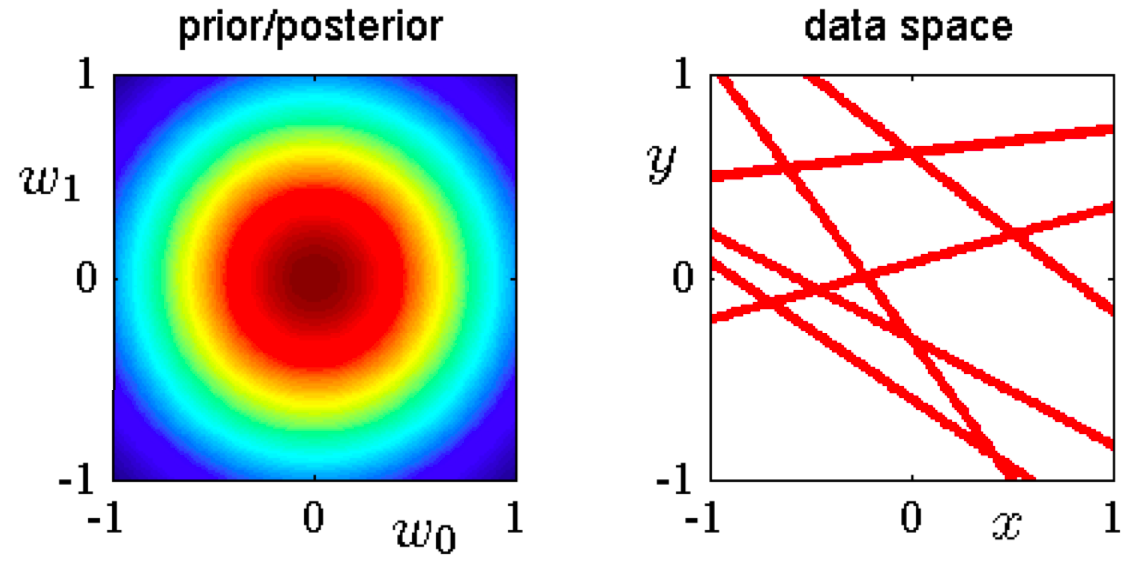
\includegraphics[width=0.6\textwidth]{figures/lin-regression-prior-PRMLFig3-7}
\par\end{center}

\begin{itemize}
\item On right,  $y(x)=\ex\left[y\mid x,w\right]=w_{0}+w_{1}x$, for randomly
chosen $w\sim p(w)=\cn\left(0,\frac{1}{2}I\right)$. 
\end{itemize}
\let\thefootnote\relax\footnotetext{\tiny{Bishop's PRML Fig 3.7}}
\end{frame}


\begin{frame}{Example in 1-Dimension: 1 Observation}
\begin{center}
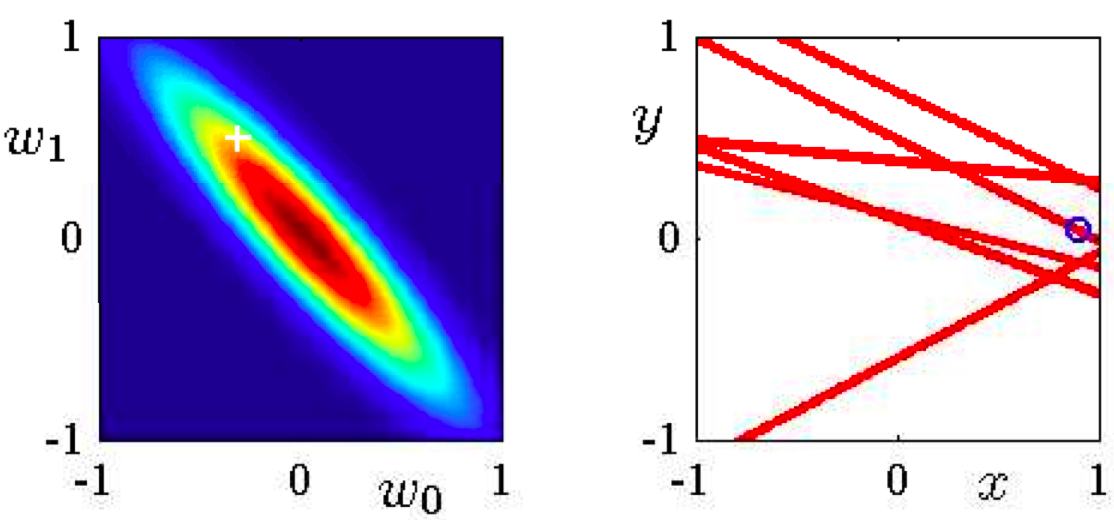
\includegraphics[width=0.6\textwidth]{{figures/lin-regression-prior-PRMLFig3-7.1pt}.png}
\par\end{center}
\begin{itemize}
\item On left: posterior distribution; white cross indicates true parameters
\item On right: 
\begin{itemize}
  \item blue circle indicates the training observation
  \item red lines,  $y(x)=\ex\left[y\mid x,w\right]=w_{0}+w_{1}x$, for randomly
  chosen $w\sim p(w | \cd )$ (posterior)
\end{itemize}
\end{itemize}

\let\thefootnote\relax\footnotetext{\tiny{Bishop's PRML Fig 3.7}}
\end{frame}
%
\begin{frame}{Example in 1-Dimension: 2 and 20 Observations}
\begin{center}
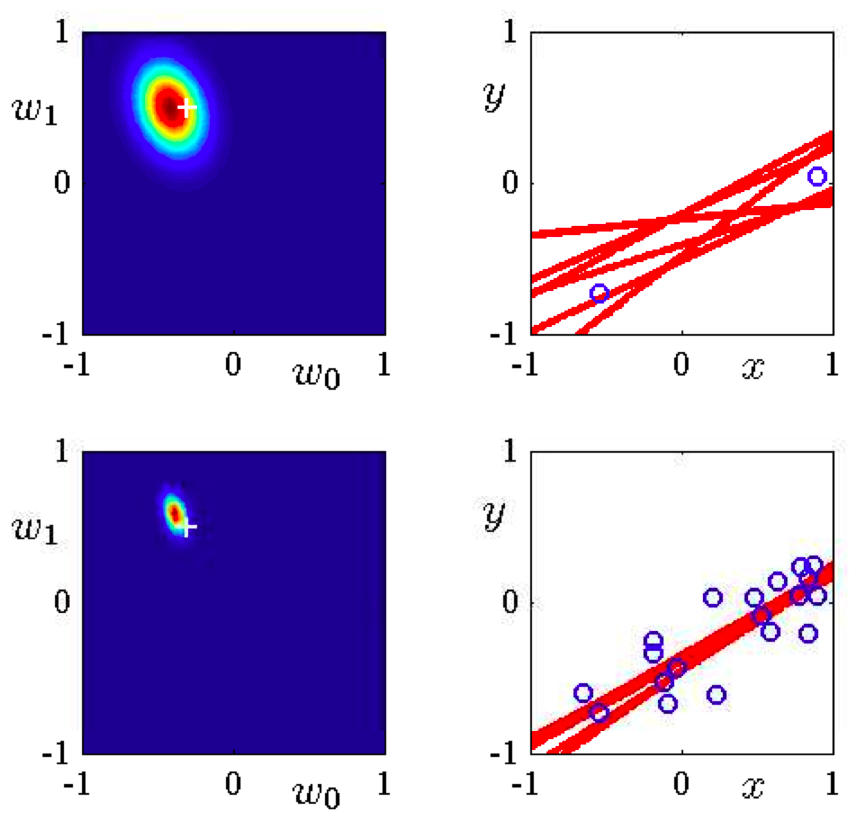
\includegraphics[height=0.7\textheight]{{figures/lin-regression-prior-PRMLFig3-7.2and20pt}.png}
\par\end{center}

\let\thefootnote\relax\footnotetext{\tiny{Bishop's PRML Fig 3.7}}
\end{frame}
%

\section{Gaussian Regression: Closed form}
\begin{frame}{Closed Form for Posterior}
\begin{itemize}
\item Model:
\begin{eqnarray*}
w & \sim & \cn\left(0,\Sigma_{0}\right)\\
\pause y_{i}\mid x,w & \text{i.i.d.} & \cn(w^{T}x_{i},\sigma^{2})
\end{eqnarray*}


\pause{}
\item Design matrix $X$ $\qquad$Response column vector $y$

\pause{}
\item \textbf{Posterior distribution is a Gaussian distribution:
\begin{eqnarray*}
w\mid\cd & \sim & \pause\cn(\mu_{P},\Sigma_{P})\\
\mu_{\text{P}} & = & \left(X^{T}X+\sigma^{2}\Sigma_{0}^{-1}\right)^{-1}X^{T}y\\
\Sigma_{\text{P}} & = & \left(\sigma^{-2}X^{T}X+\Sigma_{0}^{-1}\right)^{-1}
\end{eqnarray*}
}

\pause{}
\item \textbf{Posterior Variance} $\Sigma_{P}$ gives us a natural \textbf{uncertainty
measure.}
\end{itemize}

\end{frame}
%
\begin{frame}{Closed Form for Posterior}
\begin{itemize}
\item \textbf{Posterior distribution is a Gaussian distribution:
\begin{eqnarray*}
w\mid\cd & \sim & \pause\cn(\mu_{P},\Sigma_{P})\\
\mu_{\text{P}} & = & \left(X^{T}X+\sigma^{2}\Sigma_{0}^{-1}\right)^{-1}X^{T}y\\
\Sigma_{\text{P}} & = & \left(\sigma^{-2}X^{T}X+\Sigma_{0}^{-1}\right)^{-1}
\end{eqnarray*}
}

\pause{}
\item If we want point estimates of $w$\textbf{, MAP estimator} and the
\textbf{posterior mean} are given by
\[
\pause\hat{w}=\mu_{P}=\left(X^{T}X+\sigma^{2}\Sigma_{0}^{-1}\right)^{-1}X^{T}y
\]
 

\pause{}
\item For the prior variance $\Sigma_{0}=\frac{\sigma^{2}}{\lambda}I$,
we get
\[
\hat{w}=\mu_{P}=\left(X^{T}X+\lambda I\right)^{-1}X^{T}y,\pause
\]
which is of course the ridge regression solution. 
\end{itemize}
\end{frame}
%
\begin{comment}
\begin{frame}{Connection the MAP to Ridge Regression}
\begin{itemize}
\item The \textbf{Posterior density }on $w$\textbf{ }for\textbf{ }$\Sigma_{0}=\frac{\sigma^{2}}{\lambda}I$:\textbf{
\begin{eqnarray*}
p(w\mid\cd) & \propto & \underbrace{\exp\left(-\frac{\lambda}{2\sigma^{2}}\|w\|^{2}\right)}_{\text{prior}}\underbrace{\prod_{i=1}^{n}\exp\left(-\frac{(y_{i}-w^{T}x_{i})^{2}}{2\sigma^{2}}\right)}_{\text{likelihood}}
\end{eqnarray*}
}

\pause{}
\item To find the \textbf{MAP}, we minimize the negative log posterior:
\begin{eqnarray*}
\hat{w}_{\text{MAP}} & = & \argmin_{w\in\reals^{d}}\left[-\log p(w\mid\cd)\right]\\
\pause & = & \argmin_{w\in\reals^{d}}\underbrace{\sum_{i=1}^{n}(y_{i}-w^{T}x_{i})^{2}}_{\text{log-likelihood}}+\underbrace{\lambda\|w\|^{2}}_{\text{log-prior}}
\end{eqnarray*}


\pause{}
\item Which is the ridge regression objective.
\end{itemize}
\end{frame}
%
\begin{frame}{Predictive Posterior Distribution}
\begin{itemize}
\item Given a new input point $x_{\text{new}}$, how do we predict $y_{\text{new}}$
?

\pause{}
\item \textbf{Predictive distribution
\begin{eqnarray*}
p(y_{\text{new}}\mid x_{\text{new}},\cd) & = & \pause\int p(y_{\text{new}}\mid x_{\text{new}},w,\cd)p(w\mid\cd)\,dw\\
\pause & = & \int p(y_{\text{new}}\mid x_{\text{new}},w)p(w\mid\cd)\,dw
\end{eqnarray*}
}

\pause{}
\item For Gaussian regression, predictive distribution has closed form.
\end{itemize}
\end{frame}
%
\begin{frame}{Closed Form for Predictive Distribution}
\begin{itemize}
\item \textbf{Model}:
\begin{eqnarray*}
w & \sim & \cn\left(0,\Sigma_{0}\right)\\
\pause y_{i}\mid x,w & \text{i.i.d.} & \cn(w^{T}x_{i},\sigma^{2})
\end{eqnarray*}


\pause{ }
\item \textbf{Predictive Distribution}
\begin{eqnarray*}
p(y_{\text{new}}\mid x_{\text{new}},\cd) & = & \int p(y_{\text{new}\text{ }}\mid x_{\text{new}},w)p(w\mid\cd)\,dw.
\end{eqnarray*}

\begin{itemize}
\item Averages over prediction for each $w$, weighted by posterior distribution.

\pause{ }
\end{itemize}
\item \textbf{Closed form:}
\begin{eqnarray*}
y_{\text{new}}\mid x_{\text{new}},\cd & \sim & \cn\left(\eta_{\text{new}}\,,\,\sigma_{\text{new}}^{2}\right)\\
\pause\eta_{\text{new}} & = & \mu_{\text{P}}^{T}x_{\text{new}}\\
\pause\sigma_{\text{new}}^{2} & = & \underbrace{x_{\text{new}}^{T}\Sigma_{\text{P}}x_{\text{new}}}_{\text{from variance in }w}+\underbrace{\sigma^{2}}_{\text{inherent variance in }y}
\end{eqnarray*}
\end{itemize}
\end{frame}
%
\begin{frame}{Bayesian Regression Provides Uncertainty Estimates}
\begin{itemize}
\item With predictive distributions, we can give mean prediction with error
bands:
\end{itemize}
\begin{center}
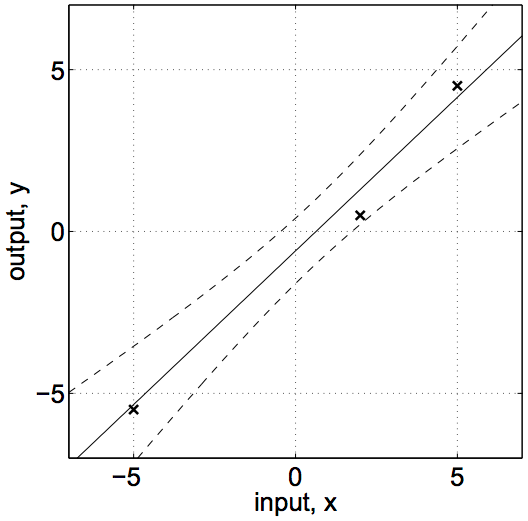
\includegraphics[height=0.7\textheight]{figures/predictiveDistWithErrorBands}
\par\end{center}

\let\thefootnote\relax\footnotetext{\tiny{Rasmussen and Williams' \emph{Gaussian Processes for Machine Learning}, Fig.2.1(b) }}
\end{frame}
\end{comment}

\end{document}

